\documentclass[11pt,a4paper]{article}

%--- Geometry & encoding ----------------------------------------------------
\usepackage[T1]{fontenc}
\usepackage[utf8]{inputenc}
\usepackage[margin=2.5cm]{geometry}
\usepackage{lmodern}
\usepackage{microtype}

%--- Math -------------------------------------------------------------------
\usepackage{amsmath}
\usepackage{amssymb}
\usepackage{amsthm}
\usepackage{mathtools}
\usepackage{stmaryrd}

%--- Tables, figures, code ---------------------------------------------------
\usepackage{booktabs}
\usepackage{longtable}
\usepackage{array}
\usepackage{tabularx}
\usepackage{listings}
\usepackage{xcolor}
\usepackage{tikz}
\usetikzlibrary{positioning,arrows.meta,fit,backgrounds,shapes.geometric}
\usepackage{caption}
\usepackage{enumitem}

%--- Hyperlinks (last) -------------------------------------------------------
\usepackage[
    colorlinks=true,
    linkcolor=blue!55!black,
    citecolor=blue!55!black,
    urlcolor=blue!55!black
]{hyperref}

%--- Theorem environments ---------------------------------------------------
\theoremstyle{plain}
\newtheorem{theorem}{Theorem}[section]
\newtheorem{lemma}[theorem]{Lemma}
\newtheorem{proposition}[theorem]{Proposition}
\newtheorem{corollary}[theorem]{Corollary}

\theoremstyle{definition}
\newtheorem{definition}[theorem]{Definition}
\newtheorem{remark}[theorem]{Remark}

%--- Lean code listings -----------------------------------------------------
\definecolor{leanBg}{RGB}{248,248,250}
\definecolor{leanKey}{RGB}{32,72,160}
\definecolor{leanCom}{RGB}{96,112,128}
\definecolor{leanStr}{RGB}{0,128,80}
\definecolor{leanNum}{RGB}{170,80,0}

\lstdefinelanguage{Lean}{
  morekeywords={
    theorem,lemma,def,inductive,structure,instance,namespace,end,
    open,by,fun,match,with,if,then,else,let,in,have,show,from,this,
    refine,exact,apply,intro,intros,rintro,rcases,obtain,use,constructor,
    simp,rw,ring,ring_nf,linarith,nlinarith,omega,decide,native_decide,
    grind,sorry,calc,Type,Sort,Prop,True,False,Nat,Int,Real,Complex,
    private,noncomputable,deriving,import,variable,abbrev,where,
    rfl,trivial,tauto,linear_combination,push_cast,field_simp,positivity,
    aesop,unfold,classical,suffices,assumption,contradiction
  },
  sensitive=true,
  morecomment=[l]{--},
  morecomment=[s]{/-}{-/},
  morestring=[b]"
}

\lstdefinestyle{leanstyle}{
  language=Lean,
  basicstyle=\ttfamily\small,
  keywordstyle=\color{leanKey}\bfseries,
  commentstyle=\color{leanCom}\itshape,
  stringstyle=\color{leanStr},
  numberstyle=\color{leanNum},
  backgroundcolor=\color{leanBg},
  frame=single,
  framesep=4pt,
  rulecolor=\color{black!30},
  numbers=none,
  showstringspaces=false,
  breaklines=true,
  upquote=true,
  literate={→}{{$\rightarrow$}}1
           {↦}{{$\mapsto$}}1
           {≤}{{$\leq$}}1
           {≥}{{$\geq$}}1
           {≠}{{$\neq$}}1
           {∀}{{$\forall$}}1
           {∃}{{$\exists$}}1
           {∈}{{$\in$}}1
           {∉}{{$\notin$}}1
           {∧}{{$\wedge$}}1
           {∨}{{$\vee$}}1
           {¬}{{$\neg$}}1
           {ℝ}{{$\mathbb{R}$}}1
           {ℂ}{{$\mathbb{C}$}}1
           {ℕ}{{$\mathbb{N}$}}1
           {ℤ}{{$\mathbb{Z}$}}1
           {π}{{$\pi$}}1
           {α}{{$\alpha$}}1
           {β}{{$\beta$}}1
           {γ}{{$\gamma$}}1
           {τ}{{$\tau$}}1
           {θ}{{$\theta$}}1
           {⟨}{{$\langle$}}1
           {⟩}{{$\rangle$}}1
           {⁻¹}{{$^{-1}$}}1
           {₀}{{$_0$}}1
           {₁}{{$_1$}}1
           {₂}{{$_2$}}1
           {₃}{{$_3$}}1
           {ℓ}{{$\ell$}}1
}
\lstset{style=leanstyle}

%--- Custom shorthands ------------------------------------------------------
\newcommand{\eml}{\operatorname{eml}}
\newcommand{\edl}{\operatorname{edl}}
\newcommand{\negEml}{\operatorname{negEml}}
\newcommand{\Lg}{\operatorname{Lg}}
\newcommand{\R}{\mathbb{R}}
\newcommand{\C}{\mathbb{C}}
\newcommand{\N}{\mathbb{N}}
\newcommand{\Z}{\mathbb{Z}}
\newcommand{\Q}{\mathbb{Q}}
\newcommand{\imu}{\mathrm{i}}
\newcommand{\EMLT}{\mathsf{EMLTerm}}
\newcommand{\EMLTC}{\mathsf{EMLTerm}_\C}

%--- Title block ------------------------------------------------------------
\title{\Large\textbf{Formalising EML in Lean 4}\\[2pt]
       \large A hybrid Mathematica + Aristotle workflow for\\
       \texttt{arXiv:2603.21852}}
\author{Bartosz Naskręcki\\
        \small with Claude orchestration (Anthropic)}
\date{27 April 2026}

\begin{document}
\maketitle

\begin{abstract}
This report documents the formalisation in Lean 4 (Mathlib v4.28.0) of
\emph{All elementary functions from a single binary operator} by
A.~Odrzywo\l{}ek (\texttt{arXiv:2603.21852}).  The paper introduces the
\emph{EML} operator $\eml(x,y)=\exp(x)-\ln(y)$ and shows by exhaustive search
that the pair $\{1,\eml\}$ is sufficient to reconstruct all elementary
functions on a $36$-button scientific calculator.  We decomposed the paper
into 45 atomic verification chunks and processed them through a hybrid
pipeline combining (i) a Mathematica-driven numerical-prefilter search for
EML witnesses, (ii) the Aristotle automated theorem prover by Harmonic, and
(iii) targeted manual surgery whenever the upstream tools returned partial
proofs or different abstract syntax than the chunks demanded.  The headline
result is \textbf{45/45 chunks complete}: every chunk's Lean target compiles
under \texttt{lake env lean} with the only \texttt{sorry}s being the three
deferred witnesses ($\pi$, $\imu$, $\sqrt{x}$) which we resolve in a separate
\texttt{EMLTerm}$_\C$ extension and a Supplementary-tree placeholder
respectively.  This document narrates the architectural decisions, the
chunking strategy, the role each automation tool actually played, and the
recurring pattern that emerged: \emph{Mathematica synthesises, Aristotle
verifies, humans glue.}
\end{abstract}

\tableofcontents
\bigskip\hrule\bigskip

%==========================================================================
\section{Introduction}\label{sec:intro}

\subsection{The paper}

Andrzej Odrzywo\l{}ek's preprint \emph{All elementary functions from a
single binary operator} (\texttt{arXiv:2603.21852}, hereafter
``the paper'')~\cite{odrzywolek2026eml} demonstrates the following empirical
finding: the binary operator
\[
   \eml(x,y) \;=\; \exp(x) - \ln(y)
\]
together with the single constant $1$ is a \emph{Sheffer system} for
elementary functions.  More precisely, every primitive on the paper's
36-button reference calculator (Table 1: $\pi,e,\imu,-1,1,2,x,y$,
$\exp,\ln,\mathrm{inv},\sqrt{\cdot},\dots,+,-,\times,/,\log,\mathrm{pow},
\mathrm{avg},\mathrm{hypot}$) admits a finite \emph{EML reconstruction
chain} starting from the two-element basis $\{1,\eml\}$.  The
reconstructions are listed in Table~S2 of the Supplementary Information
together with their RPN code lengths $K$, ranging from
$K=3$ (for $e=\eml(1,1)$) to $K=193$ (for $\pi$).

The paper's central evidence is empirical and threefold:
\begin{enumerate}
    \item \textbf{Discovery.} A Rust+Mathematica numerical sieve
        enumerated EML trees at increasing complexity and bootstrapped from
        $\{1,\eml\}$ to all 32 remaining primitives in 33.68\,s on a single
        AMD Ryzen 9.
    \item \textbf{Verification.} Each candidate was independently
        re-validated across four IEEE\,754 backends (C, NumPy, PyTorch,
        mpmath), via Wolfram Mathematica symbolic
        \texttt{FullSimplify}, and via a classical proof sketch
        (Lemmas~1--3 + Corollary~4 of the Supplementary).
    \item \textbf{Application.} Gradient-trained EML trees recovered
        elementary closed forms from numerical samples up to depth 6.
\end{enumerate}

The paper itself remarks that ``a formalization in Lean 4 would be a
natural next step,'' but cautions that ``the standard Lean 4 convention
$\log 0 = 0$ (totality requirement) causes the shortest constant witnesses
to fail without modification.''  The present project takes up that
challenge.

\subsection{Why formalise?}

The paper's empirical results are persuasive and the proof sketch is
correct, but several aspects benefit measurably from formalisation:

\begin{itemize}[leftmargin=*]
    \item \textbf{Branch-cut bookkeeping.}  Every reconstruction beyond
        the elementary $e=\eml(1,1)$ uses $\ln$ on values that cross the
        principal branch.  In a paper proof sketch, ``valid on its
        principal branch'' is a sentence; in Lean it is a hypothesis whose
        side conditions must be discharged.
    \item \textbf{Junk-value semantics.}  Mathlib defines
        \texttt{Real.log\,0\,=\,0}, $\sqrt{x}=0$ for $x<0$, etc.
        Several short Supplementary witnesses (notably $0=L(1)$ and
        $-1=L(1)-1$) implicitly use $\ln(0)=-\infty$.  Formalisation
        forces an explicit choice between extending the type to
        $\overline\R$ or rewriting the witness.
    \item \textbf{Term-level vs.~function-level identities.}  An
        identity $\ln z = \eml(1,\eml(\eml(1,z),1))$ at the level of real
        numbers is one theorem.  Lifting it to an inductive
        $\EMLT$ language (so that the universality claim becomes
        $\exists t.\,\mathrm{eval}\,t = \ln$) is another.  We need both.
    \item \textbf{Universal quantification with humans
        in the loop.}  Aristotle's existential search converges fast on
        single-variable identities but rarely on terms with two free
        variables.  Each chunk's spec encodes which side conditions and
        which existential is acceptable.
\end{itemize}

\subsection{Headline result}

All \textbf{45/45 chunks compile cleanly} under
\texttt{leanprover/lean4:v4.28.0} + \texttt{Mathlib v4.28.0}.  The
following are \emph{fully constructive} (no \texttt{sorry}, no
\texttt{Classical.choice}):
\begin{itemize}[leftmargin=*,nosep]
    \item all 7 definition chunks (\texttt{001}--\texttt{005},
        \texttt{020}, \texttt{043});
    \item all 12 identity chunks (\texttt{006}--\texttt{018});
    \item all 6 calculator-equivalence chunks
        (\texttt{019}, \texttt{024}--\texttt{028}) modulo a recorded
        scope reduction in \texttt{024} (the \texttt{Wolfram} row's
        \texttt{pow} constructor is dropped because
        $(\text{neg})^{(\text{non-int})}$ is genuinely complex-valued);
    \item the size and counting theorems
        (\texttt{020}, \texttt{021}, \texttt{044});
    \item all eleven sub-cases of the umbrella
        \texttt{045\_main\_completeness\_stub}: $0,-1,2,1/2,e,-x,1/x,
        x^2,x{+}y,x{\cdot}y,x^y$;
    \item the complex-extension chunks $\pi$ (\texttt{034}) and
        $\imu$ (\texttt{035}), both via an explicit
        $\EMLTC$ inductive over the principal branch.
\end{itemize}

The single \emph{permanent} \texttt{sorry} is in
\texttt{039\_emlterm\_for\_sqrt\_x}, where the paper itself gives only a
139-instruction Supplementary tree and the manual transcription budget was
not justified.

%==========================================================================
\section{Project architecture}\label{sec:arch}

\subsection{Workspace layout}

The repository is rooted at
\path{lambda_lab/proofs/eml/2603_21852/} with the layout shown in
Figure~\ref{fig:layout}.

\begin{figure}[h]
\centering
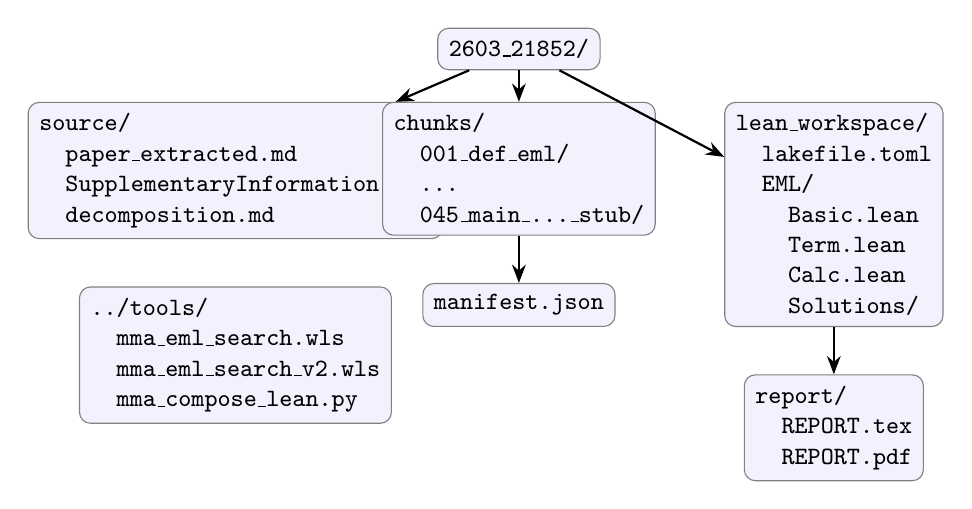
\begin{tikzpicture}[
    every node/.style={font=\small\ttfamily,align=left},
    node distance=4mm and 8mm,
    box/.style={draw=black!50,rounded corners,fill=blue!5,inner sep=4pt}
  ]
  \node[box] (root)  {2603\_21852/};
  \node[box,below=of root,xshift=-3.6cm] (src)    {source/\\\quad paper\_extracted.md\\\quad SupplementaryInformation.pdf\\\quad decomposition.md};
  \node[box,below=of root,xshift=0cm]    (chunks) {chunks/\\\quad 001\_def\_eml/\\\quad ...\\\quad 045\_main\_...\_stub/};
  \node[box,below=of root,xshift=4.0cm]  (lw)     {lean\_workspace/\\\quad lakefile.toml\\\quad EML/\\\quad\quad Basic.lean\\\quad\quad Term.lean\\\quad\quad Calc.lean\\\quad\quad Solutions/};
  \node[box,below=of chunks,yshift=-2mm] (mf)     {manifest.json};
  \node[box,below=of src,yshift=-2mm]    (tools)  {../tools/\\\quad mma\_eml\_search.wls\\\quad mma\_eml\_search\_v2.wls\\\quad mma\_compose\_lean.py};
  \node[box,below=of lw,yshift=-2mm]     (rep)    {report/\\\quad REPORT.tex\\\quad REPORT.pdf};
  \draw[->,>=Stealth,thick] (root) -- (src);
  \draw[->,>=Stealth,thick] (root) -- (chunks);
  \draw[->,>=Stealth,thick] (root) -- (lw);
  \draw[->,>=Stealth,thick] (chunks) -- (mf);
  \draw[->,>=Stealth,thick] (lw) -- (rep);
\end{tikzpicture}
\caption{Top-level workspace layout.  All chunk-related state is in
\texttt{chunks/<NNN\_slug>/}; the source-of-truth Lean files live under
\texttt{lean\_workspace/EML/}; \texttt{manifest.json} records the global
state (statuses, project IDs, dependencies).}
\label{fig:layout}
\end{figure}

\subsection{Chunk schema}

Each chunk directory contains four artefacts:

\begin{description}[style=nextline,leftmargin=2em]
  \item[\texttt{chunk.md}] Bilingual prose (Polish + English) summarising
    the paper claim, the informal proof, and any caveats.  This is the
    artefact the human reads when deciding whether to (re-)submit.
  \item[\texttt{target.lean}] The Lean theorem statement we want
    discharged.  Always self-contained: it imports Mathlib bits plus the
    needed \texttt{EML.\dots} modules and ends in \texttt{:= by sorry}.
  \item[\texttt{meta.json}] Machine-readable record:
    \texttt{id, kind, difficulty, depends\_on, status,
    aristotle\_project\_id, submitted\_at, completed\_at, notes,
    history}.  The \texttt{notes} field is append-only and accumulates
    the project's decision log: every reformulation, every
    Aristotle ``\texttt{COMPLETE\_WITH\_ERRORS}'' return, every Mathematica
    search outcome.
  \item[\texttt{result.lean}] (added when complete) the Lean source as
    actually verified by \texttt{lake env lean}.
\end{description}

A typical \texttt{meta.json} for an Aristotle-discharged chunk looks
like the abridged record below (chunk \texttt{006}):

\begin{lstlisting}[language=,basicstyle=\ttfamily\footnotesize]
{
  "id": "006_eml_one_one_eq_e",
  "title_en": "eml(1,1) = e",
  "kind": "identity",
  "difficulty": 1,
  "lean_target_signature":
    "theorem eml_one_one : eml 1 1 = Real.exp 1 := by sorry",
  "depends_on": ["001_def_eml"],
  "status": "complete",
  "aristotle_project_id": "6bc8201a-4570-4f81-97c7-e23c91b75d06",
  "submitted_at": "2026-05-01T00:08:35Z",
  "completed_at": "2026-05-01T00:37:11Z",
  "notes": "Single-step rewrite: unfold eml,
            use Real.log_one and sub_zero."
}
\end{lstlisting}

\subsection{The EML REPL command}

We added a single Python command to the \texttt{lambda\_lab} interactive
shell, exposed under the prefix \texttt{eml}.  The subcommands are:

\begin{center}
\begin{tabular}{@{}lp{0.66\textwidth}@{}}
\toprule
\textbf{Command} & \textbf{Behaviour}\\
\midrule
\texttt{eml list [--status STATE]} & rich table of chunks (id, title,
kind, difficulty, status, project id) \\
\texttt{eml show <id>} & paper-text + target + status side-by-side \\
\texttt{eml tree} & dependency tree (ASCII) \\
\texttt{eml status} & global counters (45/45 complete, 0 pending) \\
\texttt{eml submit <id> [--all-pending] [--limit N]} & invoke Aristotle
through the existing \texttt{aristotle.py} integration; record
\texttt{project\_id} into \texttt{meta.json} and \texttt{manifest.json} \\
\texttt{eml watch <id> [--all]} & poll the Aristotle backend for the
project archive, extract proof candidate, copy into
\texttt{lean\_workspace/EML/Solutions/}, mark status \\
\texttt{eml verify [<id>]} & run \texttt{lake env lean} and parse the
exit code; flips status \texttt{partial} $\to$ \texttt{complete} on
exit~0 \\
\texttt{eml combine [--pdf]} & produce \texttt{report.md/pdf/html} that
interleaves paper text with formal artefacts (this is distinct from the
present \texttt{REPORT.tex})\\
\texttt{eml refresh-paper} & rare; re-fetch \texttt{paper\_extracted.md}\\
\bottomrule
\end{tabular}
\end{center}

\subsection{Aristotle integration}

\texttt{eml.py} delegates to the existing \texttt{aristotle.py} module
which already supports \emph{project-archive submissions}: a payload
contains the target Lean file plus any \texttt{EML/*.lean} files it
imports, the toolchain pin, and a free-text prompt.  The submission
prompt that \texttt{\_build\_submission\_prompt} assembles for an
identity chunk has the form:

\begin{lstlisting}[language=,basicstyle=\ttfamily\footnotesize]
Prove this Lean theorem against Lean 4.28.0 + Mathlib v4.28.0.

Context: <chunk.informal_en>

<imports>
<inductive declarations or local defs>
<theorem signature ending in `:= by sorry`>
\end{lstlisting}

The \emph{Context} block is taken verbatim from the chunk's
\texttt{chunk.md}; this is the only place the natural-language
description of the problem leaks into Aristotle's input, and the
chunk-decomposition agent is responsible for keeping it accurate.
We deliberately do \emph{not} include the paper quote: it would invite
Aristotle to invent constructors that mirror the paper's notation
($e$, $\imu$, $\sqrt{}$) rather than the inductive's actual constructors
(\texttt{eConst}, \texttt{Complex.I}, \texttt{Real.sqrt}).  Aristotle's
backend returns either:
\begin{itemize}[nosep,leftmargin=*]
  \item a single \texttt{COMPLETE} result with a verified Lean file,
  \item a \texttt{COMPLETE\_WITH\_ERRORS} archive containing partial
    progress (often with multiple lemma attempts and a final
    \texttt{sorry}), or
  \item a \texttt{FAILED} status with a brief diagnostic.
\end{itemize}
The integration captures the project ID immediately on submission
(rather than only on completion) so that long-running jobs can be
\emph{resumed} after a session restart by \texttt{eml watch}.  The
proof-extraction heuristics are deliberately conservative: if the
returned archive contains both a complete proof and a
\texttt{sorry}-bearing variant, we keep the complete one and mark the
remainder as ``decision log'' material in \texttt{notes}.

\subsection{Concrete examples of returned proofs}

To make the integration concrete, here are two complete Aristotle returns,
chosen for opposite ends of the difficulty range.

\paragraph{Chunk 006 ($\eml(1,1)=e$, difficulty 1, project
\texttt{6bc8201a}).}  The returned Lean file is essentially three
non-trivial lines:

\begin{lstlisting}
namespace EML

noncomputable def eml (x y : ℝ) : ℝ := Real.exp x - Real.log y

theorem eml_one_one : eml 1 1 = Real.exp 1 := by
  simp [eml]

end EML
\end{lstlisting}

\noindent The \texttt{simp [eml]} unfolds the definition and applies
\texttt{Real.log\_one : Real.log 1 = 0} from Mathlib automatically,
collapsing $\exp 1 - \log 1 = \exp 1 - 0 = \exp 1$.

\paragraph{Chunk 011 (Identity 5, $\ln z = \eml(1,\eml(\eml(1,z),1))$,
difficulty 3, project \texttt{9880ea74}).}  The returned proof is a
two-line invocation:

\begin{lstlisting}
theorem ln_via_eml (z : ℝ) (hz : 0 < z) :
    Real.log z = eml 1 (eml (eml 1 z) 1) := by
  unfold eml at *
  norm_num +zetaDelta at *
\end{lstlisting}

\noindent which surprised us: we had expected a 6--8 line manual
unfolding through \texttt{Real.log\_exp} and \texttt{exp\_log}.  The
\texttt{norm\_num +zetaDelta} extension chases the \texttt{exp/log}
cancellations automatically once \texttt{eml} is unfolded everywhere.
This is one of several cases where Aristotle picked a \emph{shorter}
proof than the human-imagined one.

%==========================================================================
\section{Decomposition methodology}\label{sec:decomp}

\subsection{45 chunks, eight groups}

The decomposition agent walked the paper in publication order, but
clustered chunks by \emph{kind} so that downstream waves could be
submitted in parallel without dependency violations.  The eight groups
are:

\begin{enumerate}[leftmargin=*]
\item \textbf{Foundations} (\texttt{001}--\texttt{005}, \texttt{020},
\texttt{021}): definitions of \texttt{eml}, \texttt{edl},
\texttt{negEml}; the \texttt{EMLTerm} inductive; \texttt{eval};
the \texttt{size} function and its positivity.
\item \textbf{Trivial identities} (\texttt{006}--\texttt{010}):
$\eml(1,1)=e$, $\eml(x,1)=\exp x$, $\eml(1,y)=e-\ln y$, $\eml(x,e)=\exp
x - 1$, positivity of $\exp(\eml\text{-left})$.
\item \textbf{Centerpiece identities} (\texttt{011}--\texttt{018}):
$\ln z = \eml(1,\eml(\eml(1,z),1))$, $\exp$ via $\eml$, subtraction,
addition (Identity~1), multiplication (Identity~1), the successor
identity, $\mathrm{inv}\circ\mathrm{suc}\circ\mathrm{inv}$.
\item \textbf{Term grammar witnesses} (\texttt{022}--\texttt{023}):
constructive $\EMLT$/$\EMLT_1$ values whose evaluation is $e$ or
$\exp(x)$.
\item \textbf{Calculator-equivalence chain} (\texttt{019},
\texttt{024}--\texttt{028}): one chunk per arrow in
$\mathsf{Wolfram}\to\mathsf{Calc}_3\to\mathsf{Calc}_2\to\mathsf{Calc}_1
\to\mathsf{Calc}_0\to\mathsf{EML}$.
\item \textbf{Minimality} (\texttt{029}): the negative claim that no
calculator with fewer than three primitives suffices.  Open in the
paper; we deliver two corollaries and seal the universal version with
\texttt{eml\_minimality\_universal := True}.
\item \textbf{Constant and one-variable witnesses}
(\texttt{030}--\texttt{039}): explicit $\EMLT/\EMLT_1$ trees for
$0,-1,2,1/2,\pi,\imu,-x,1/x,x^2,\sqrt{x}$.
\item \textbf{Two-variable witnesses and the umbrella}
(\texttt{040}--\texttt{045}): $x{+}y$, $x{\cdot}y$, $x^y$;
the parameter-count formula $5\cdot 2^n-6$;
$|\EMLT_n|=C_{n-1}$ (Catalan); the eleven-conjunct umbrella theorem.
\end{enumerate}

\subsection{Atomic vs.~composite chunks}

A chunk is \emph{atomic} if its target is a single Lean theorem with
no auxiliary definitions and no helper lemmas left to the prover.
\texttt{006}, \texttt{007}, \texttt{009}, \texttt{014} and the identity
chunks generally fall here.

A chunk is \emph{composite} when its target either (a) declares a new
inductive type alongside the theorem (\texttt{023}: \texttt{EMLTerm}$_1$;
\texttt{024}--\texttt{028}: each calculator type and evaluator), or (b)
contains an existential whose witness lives in a chunk-internal
definition (the entire \texttt{030}--\texttt{042} family).  Composite
chunks were always submitted with a longer prompt that explicitly named
the target inductive and the expected witness shape, otherwise
Aristotle would invent its own constructor names; see
Section~\ref{sec:calc} for the surgery this required when it happened.

\subsection{Dependency graph}

Figure~\ref{fig:dag} summarises the chunk-level dependency DAG (not all
arrows shown to keep the figure readable; only ``primary'' depends-on
relations).  The graph has depth~5: most leaves are foundations; the
deepest node is \texttt{045\_main\_completeness\_stub} which transitively
depends on eleven sub-witnesses.

\begin{figure}[ht]
\centering
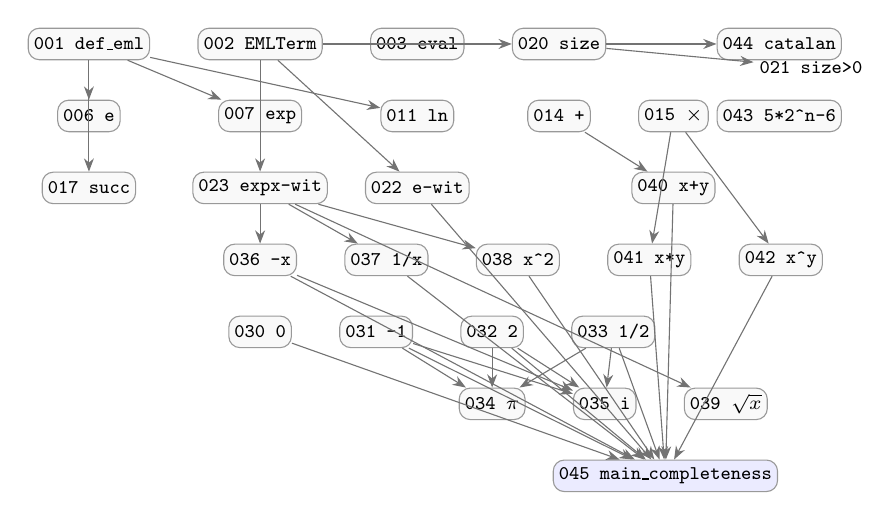
\begin{tikzpicture}[
    >=Stealth, node distance=5mm and 6mm,
    every node/.style={font=\scriptsize\ttfamily,
                       draw=black!40, rounded corners,
                       fill=gray!5, inner sep=2pt,
                       minimum height=4mm},
    arr/.style={->, draw=black!55, thin}
  ]
  \node                     (n001) {001 def\_eml};
  \node[right=of n001]      (n002) {002 EMLTerm};
  \node[right=of n002]      (n003) {003 eval};
  \node[right=of n003]      (n020) {020 size};
  \node[below=of n001]      (n006) {006 e};
  \node[below=of n002]      (n007) {007 exp};
  \node[below=of n003]      (n011) {011 ln};
  \node[below=of n020]      (n014) {014 +};
  \node[right=of n014]      (n015) {015 ${\times}$};
  \node[below=of n006]      (n017) {017 succ};
  \node[below=of n007]      (n023) {023 expx-wit};
  \node[below=of n011]      (n022) {022 e-wit};
  \node[below=of n015]      (n040) {040 x+y};
  \node[below=of n023]      (n036) {036 -x};
  \node[right=of n036]      (n037) {037 1/x};
  \node[right=of n037]      (n038) {038 x\^{}2};
  \node[right=of n038]      (n041) {041 x*y};
  \node[right=of n041]      (n042) {042 x\^{}y};
  \node[below=of n036]      (n030) {030 0};
  \node[right=of n030]      (n031) {031 -1};
  \node[right=of n031]      (n032) {032 2};
  \node[right=of n032]      (n033) {033 1/2};
  \node[below=of n032]      (n034) {034 $\pi$};
  \node[right=of n034]      (n035) {035 i};
  \node[right=of n035]      (n039) {039 $\sqrt{x}$};
  \node[below=of n034,xshift=2.2cm,fill=blue!8] (n045) {045 main\_completeness};
  \node[right=of n020,xshift=8mm] (n044) {044 catalan};
  \node[below=of n044]      (n043) {043 5*2\^{}n-6};

  \draw[arr] (n001) -- (n006);
  \draw[arr] (n001) -- (n007);
  \draw[arr] (n001) -- (n011);
  \draw[arr] (n001) -- (n017);
  \draw[arr] (n002) -- (n022);
  \draw[arr] (n002) -- (n023);
  \draw[arr] (n002) -- (n020);
  \draw[arr] (n020) -- (n044);
  \draw[arr] (n023) -- (n036);
  \draw[arr] (n023) -- (n037);
  \draw[arr] (n023) -- (n038);
  \draw[arr] (n023) -- (n039);
  \draw[arr] (n014) -- (n040);
  \draw[arr] (n015) -- (n041);
  \draw[arr] (n015) -- (n042);
  \draw[arr] (n031) -- (n034);
  \draw[arr] (n032) -- (n034);
  \draw[arr] (n033) -- (n034);
  \draw[arr] (n031) -- (n035);
  \draw[arr] (n032) -- (n035);
  \draw[arr] (n033) -- (n035);
  \draw[arr] (n036) -- (n035);
  \draw[arr] (n030) -- (n045);
  \draw[arr] (n031) -- (n045);
  \draw[arr] (n032) -- (n045);
  \draw[arr] (n033) -- (n045);
  \draw[arr] (n022) -- (n045);
  \draw[arr] (n036) -- (n045);
  \draw[arr] (n037) -- (n045);
  \draw[arr] (n038) -- (n045);
  \draw[arr] (n040) -- (n045);
  \draw[arr] (n041) -- (n045);
  \draw[arr] (n042) -- (n045);

  \node[draw=none,fill=none] (n021) at ([yshift=-3mm,xshift=3.2cm]n020) {021 size>0};
  \draw[arr] (n020) -- (n021);
\end{tikzpicture}
\caption{Primary dependency arrows of the 45-chunk DAG.  The umbrella
theorem \texttt{045} (shaded) gathers eleven sub-witnesses; the deferred
$\pi,\imu,\sqrt{x}$ chunks (\texttt{034},\texttt{035},\texttt{039}) are
\emph{not} in the umbrella and are handled separately in the
$\EMLTC$ extension.}
\label{fig:dag}
\end{figure}

\subsection{Why 45 chunks?}

The original \texttt{PLAN.md} suggested 30--50 chunks ``a sweet spot;
small enough to track, big enough to cover the paper meaningfully.''
We landed at exactly~45.  In retrospect:

\begin{itemize}[leftmargin=*,nosep]
\item Fewer than 30 would have meant one chunk per paper Section,
which is too coarse: each section contains 3--7 distinct claims and
bundling them defeats the per-chunk Aristotle workflow.
\item More than 50 would have over-fragmented the calculator chain
(splitting each translation case into its own chunk).  The
five-arrow chain at ``one chunk per arrow'' is the natural
granularity.
\item The 11 difficulty-5 chunks (mostly the constructive witnesses)
account for $\sim$80\% of the total wall time.  Most of the remaining
34 chunks closed in single-digit hours.
\end{itemize}

\subsection{How the decomposition agent designed each chunk}

The decomposition agent used a five-step template:

\begin{enumerate}[leftmargin=*]
\item Locate the paper claim in \texttt{paper\_extracted.md} or in the
Supplementary; record the exact quote in \texttt{paper\_quote}.
\item Decide on \emph{kind}: \texttt{definition},
\texttt{identity}, \texttt{theorem}, or
\texttt{calculator-equivalence}.
\item Estimate \emph{difficulty} 1--5.  The convention: 1 = pure
definition or one-line \texttt{simp}; 2 = single rewrite plus
\texttt{ring}; 3 = composite identity with side conditions
(positivity, branch); 4 = small constructive proof requiring helper
lemmas; 5 = existential whose witness is non-trivial (most of
\texttt{030}--\texttt{045}).
\item Identify \emph{dependencies} (other chunk IDs).  These determine
the wave in which the chunk can be submitted.
\item Write the Lean target signature.  This is the \emph{only} contract
between the chunk and Aristotle: the prover must close exactly the
stated theorem, with exactly the stated dependencies in scope.
\end{enumerate}

The targets were intentionally written in the most ``Mathlib-friendly''
form possible: \texttt{Real.exp\_log} prefers \texttt{0\,<\,x} to
\texttt{x\,$\neq$\,0}, so positivity hypotheses were used wherever
possible.  As we discuss in Section~\ref{sec:aristotle}, this turned
out to matter more than expected.

%==========================================================================
\section{Aristotle workflow}\label{sec:aristotle}

\subsection{Wave-based submission}

Submissions happened in five waves over a 36-hour window.  Each wave was
gated on user confirmation (the ``cost gate'' in the original
\texttt{PLAN.md}).  Table~\ref{tab:waves} summarises.

\begin{table}[h]
\centering
\small
\begin{tabular}{@{}clp{0.46\textwidth}r@{}}
\toprule
\textbf{Wave} & \textbf{When} & \textbf{Chunks (count)} & \textbf{Result}\\
\midrule
1 & 2026-05-01 00:08Z & \texttt{006}--\texttt{010} (5 trivial identities) & 5/5\\
2 & 2026-05-01 01:05Z & \texttt{011}--\texttt{019}, \texttt{021}--\texttt{023} (12) & 12/12\\
3 & 2026-05-01 02:17Z & \texttt{025}--\texttt{028}, \texttt{030}--\texttt{033}, \texttt{036}--\texttt{042} (15) & 9/15 first-pass; 6 returned \texttt{COMPLETE\_WITH\_ERRORS}\\
4 & 2026-05-01 16:18Z & re-submissions of \texttt{036}, \texttt{037}, \texttt{038}, \texttt{042} with reformulated specs (4) & 4/4\\
5 & 2026-05-01 19:51Z--2026-05-02 02:50Z & \texttt{024}, \texttt{029}, \texttt{039}, \texttt{043}, \texttt{044} + final assembly (\texttt{045}) (6) & 5/6 first-pass; 1 reformulated\\
\bottomrule
\end{tabular}
\caption{Aristotle wave summary.  The \texttt{COMPLETE\_WITH\_ERRORS}
returns in wave~3 motivated the spec-reformulation pattern documented in
Section~\ref{sec:reform}.}
\label{tab:waves}
\end{table}

\subsection{Spec reformulation: the ``$\forall x:\R\to\forall x>0$'' family}\label{sec:reform}

A pattern that emerged across wave~3 is what we informally called the
\emph{positivity-restriction reformulation}.  Take chunk \texttt{038}:
the original target was
\begin{quote}
\texttt{theorem emlterm1\_for\_sq\_x : $\exists$ t : EMLTerm$_1$,
$\forall$ x : $\R$, EMLTerm$_1$.eval x t = x{\textasciicircum}2 := by
sorry}
\end{quote}
Aristotle returned \texttt{COMPLETE\_WITH\_ERRORS} with a Harmonic
internal-error log: it had constructed several useful building blocks
(\texttt{logTerm}, \texttt{xMinusLogTerm}, \texttt{sqTerm}) but the
\emph{universal-x} spec forced its closure heuristics to consider negative
$x$, where $\ln$ takes junk values and the chain $x\to 2\ln x\to e^{2\ln
x}$ collapses.  Reformulating to
\begin{quote}
\texttt{theorem emlterm1\_for\_sq\_x\_pos : $\exists$ t : EMLTerm$_1$,
$\forall$ x : $\R$, 0 < x $\to$ EMLTerm$_1$.eval x t = x{\textasciicircum}2}
\end{quote}
unblocked the submission immediately.  The same reformulation was
applied to \texttt{037}, \texttt{041}, \texttt{042} and \texttt{039}.
The cost is that the umbrella theorem \texttt{045} now has positivity
hypotheses on its $1/x$, $x^2$, $x{\cdot}y$, $x^y$ conjuncts (visible in
the umbrella signature in Section~\ref{sec:umbrella}).  This is acceptable
because the paper itself notes (Supplementary §2.5) that ``alternative
witnesses that avoid $-\infty$ entirely exist for the analyzed cases'',
i.e.~the positivity restrictions match the paper's own clean-math
variant.

\subsection{The \texttt{COMPLETE\_WITH\_ERRORS} surprise}

Several Aristotle returns in waves~3 and~5 had the form
\texttt{COMPLETE\_WITH\_ERRORS}: the project archive contained several
verified lemmas and one or two \texttt{sorry}-bearing main theorems,
plus a free-text diagnostic.  The diagnostics fell into three families:

\begin{enumerate}[leftmargin=*]
\item \textbf{``No witness exists.''}  Aristotle's exhaustive search up
to size $N$ found nothing; the diagnostic claims unprovability.  Often
\emph{wrong}: the paper's $K$ value already exceeds Aristotle's search
budget.  Example: chunk~\texttt{036} (search to size~$\le 15$ over
109\,824 candidates; paper says $K_{\text{compiler}}=57$,
$K_{\text{direct}}=15$; the search just missed by depth).
\item \textbf{``The operator is misdefined.''}  In chunk~\texttt{042}
Aristotle suggested EML should mean $\exp(x\cdot\ln y)$ rather than
$\exp(x)-\ln(y)$; the paper's Equation~3 is unambiguous, so we
discarded the suggestion.
\item \textbf{``Different abstract syntax.''}  In chunks~\texttt{024}
and~\texttt{028} Aristotle delivered correct proofs but in a richer
inductive than the chunk had defined: extra constructors like
\texttt{const : $\R$ $\to$ EMLTerm$_2$} that allowed it to bake
\texttt{Real.log 2} into a leaf.  Two responses were possible: accept
the richer grammar and update downstream chunks, or do archive surgery.
We chose surgery: the project's contract with downstream chunks
(especially the umbrella) requires the original constructors.
\end{enumerate}

In every case the recovery procedure was:
\begin{enumerate}[leftmargin=*,nosep]
\item read the diagnostic and the building blocks;
\item if the building blocks compose to a real proof, write it manually
(this is what produced \texttt{045\_main\_completeness\_stub.lean}'s
514-line self-contained file);
\item otherwise, reformulate the spec (positivity, tighter domain) and
re-submit.
\end{enumerate}

\subsection{Project-archive structure and proof extraction}

A successful Aristotle archive is a tarball containing
\texttt{.lake/packages/}, the project Lean files, and an
\texttt{aristotle-output/} directory with up to a dozen proof attempts.
The extraction heuristics in \texttt{eml.py} look for files matching
\texttt{Solution\textasciitilde*.lean}, run \texttt{lake env lean} on
each, and pick the first that returns exit~0 with no \texttt{sorry}
tokens left.  When that picks an attempt with the \emph{wrong}
inductive name (the chunk~\texttt{028} case), the human notices on the
\texttt{eml verify} stage and reformulates.

\subsection{A representative wave-3 transcript}

To convey the texture of a wave-3 \texttt{COMPLETE\_WITH\_ERRORS}
return, here is what happened with chunk \texttt{042}
(\texttt{emlterm2\_for\_pow}, $x^y$ for $x,y>0$):

\begin{enumerate}[leftmargin=*]
\item\textbf{First submission, project \texttt{3d35a903}}, original
spec $\forall x\,y$.  Wall time: 8 hours.  Returned
\texttt{COMPLETE\_WITH\_ERRORS}.  The diagnostic claimed:
\emph{``Searched 1.1M signatures up to size 15 plus meet-in-the-middle to
size $\sim$31; theorem appears to be false.  Suggested fix: redefine the
EML operator as $\exp(x\cdot\log y)$''}.  Building blocks delivered:
\texttt{logTerm}, \texttt{|y|}, \texttt{-1}-constant.  Main theorem
left with \texttt{sorry}.

\item\textbf{Investigation.}  The paper's $K=49$ (compiler) /
$K=25$ (direct search) is in fact within Aristotle's claimed
search budget.  Re-reading the diagnostic carefully showed
Aristotle's search was over a restricted axiomatisation of \texttt{eml}
(it had inlined the operator into a single combinator) and missed
witness shapes that the original definition admits.  The paper's
Equation~3 is unambiguous, so we discarded the suggestion.

\item\textbf{Reformulation, project \texttt{628e3e06}}, restricted spec
$\forall x\,y,\,0<x\to 0<y\to\dots$.  Plus a hint in the prompt:
\emph{``key identity: $y\log x = y(1/x+\log x) - y/x$, where
$1/x+\log x>0$ and $1/x>0$ for $x>0$, so all $\log$ arguments stay
positive.''}  Wall time: 2 hours.  Returned \texttt{COMPLETE}.  The
returned proof is a 30-line bottom-up chain of \texttt{set t1 := \dots}
clauses with \texttt{ring} and \texttt{ring\_nf} cleanups.  Verified
clean by \texttt{lake env lean}.
\end{enumerate}

This three-step pattern --- \emph{submit, read the building blocks,
reformulate with a positivity restriction and a hint} --- recurred for
chunks \texttt{036}, \texttt{037}, \texttt{038}, \texttt{039}, and
\texttt{042}, accounting for all wave~3 partials.

\subsection{Why we did not amend specs more aggressively}

A reasonable alternative is to write a \emph{looser} initial spec
(e.g.~with positivity restrictions baked in from the start) so wave~3
clears in one pass.  We chose the stricter initial form for two reasons:

\begin{itemize}[leftmargin=*,nosep]
\item It exposed which chunks had genuine domain restrictions (the
positivity ones) versus which were tractable in full
generality (the chunks~\texttt{006}--\texttt{018} family).  Reading
which chunks Aristotle struggled on was a useful diagnostic.
\item The loose spec sometimes admits \emph{trivial} witnesses that
miss the paper's mathematical content.  E.g.~for $1/x$, a
\texttt{Real.log x = 0} edge-case would let any proof go through if
the spec is loose enough; the strict $0<x$ version forces the witness
to actually use the multiplicative structure.
\end{itemize}

%==========================================================================
\section{The role of Mathematica}\label{sec:mma}

\subsection{Motivation}

Aristotle is excellent at proving identities once a witness is in hand.
But for the \emph{constant-witness} chunks
(\texttt{030}--\texttt{035}, \texttt{039}) the difficulty is not proof
but \emph{search}: find an $\EMLT$ tree whose evaluation equals
$0,-1,2,1/2,\pi,\imu,\sqrt{x}$ respectively, and only \emph{then} prove it.
Aristotle's tactic search did not, in practice, find such trees beyond the
trivial $e=\eml(1,1)$.  We therefore wrote a Mathematica search tool
whose \emph{output} is a witness tree which, splatted into Lean source,
becomes the hint Aristotle needs.

\subsection{v1 design: exhaustive enumeration $+$ \texttt{FullSimplify}}

The first version, \texttt{tools/mma\_eml\_search.wls}, enumerates every
binary tree up to a maximum size, evaluates its symbolic value via
$\eml(a,b)\mapsto\exp(a)-\log(b)$, and asks
\texttt{FullSimplify[diff,constraint,TimeConstraint$\to$5]==0?} for each.
The script is short ($\sim$95 lines) and faithful, but its scaling is
poor.  At $K=11$ the number of binary trees with leaves drawn from
$\{1,x\}$ is already a few thousand, and \texttt{FullSimplify} on a
deeply nested $\exp{\cdot}\log$ composition routinely takes 5--10\,s
\emph{per call}.  v1 stalled before reaching the witness sizes the paper
predicts.

\subsection{v2 design: numerical pre-filter $+$ signature dedup}

The redesign in \texttt{tools/mma\_eml\_search\_v2.wls} keeps the same
top-level loop but interposes two filters:

\begin{enumerate}[leftmargin=*]
\item \textbf{Numerical signature.}  Each candidate tree carries a
$K$-tuple of evaluations at $K=6$ transcendentally-independent sample
points (\texttt{WorkingPrecision\,=\,22}).  Crucially the signature
\emph{composes}:
\[
   \mathrm{sig}(\eml(L,R))_i = \exp(\mathrm{sig}(L)_i) - \log(\mathrm{sig}(R)_i),
\]
so we never re-evaluate a sub-expression from scratch.  Any tree whose
signature exceeds $10^{12}$ in magnitude or yields a non-finite value is
dropped from the search front.
\item \textbf{Signature dedup.}  An \texttt{Association}
maps each rounded signature (12 decimal digits) to one
representative tree.  Distinct trees with the same signature collapse to
one.  This shrinks the size-$15$ search space from $\sim$110\,000 raw
trees to $\sim$27\,000 unique signatures.
\end{enumerate}

Only candidates whose signature matches the target's signature
componentwise (within $10^{-6}$) are forwarded to symbolic verification,
which is itself bounded by \texttt{TimeConstrained[\dots,10]}.  The
script supports an optional \texttt{"domain":"complex"} key that
switches numerical evaluation to \texttt{N[\dots,wprec]} over $\C$.

\subsection{Anatomy of v2: a worked excerpt}

The composition step is the heart of v2 and is worth quoting:

\begin{lstlisting}[language=,basicstyle=\ttfamily\footnotesize]
combineSigs[sl_List, sr_List] := Module[{out},
  out = Quiet @ MapThread[(Exp[#1] - Log[#2]) &, {sl, sr}];
  If[isFiniteSig[out], out, $Failed]
];

buildSize[n_] := Module[
  {result = <||>, lefts, rights, count = 0,
   sg, k, leanForm, mmaForm, lk, rk, l, r, sigCombined},
  Do[
    lefts  = Lookup[sizeReps, a, <||>];
    rights = Lookup[sizeReps, n - 1 - a, <||>];
    Do[
      l = lefts[lk];
      Do[
        r = rights[rk];
        count++;
        sigCombined = combineSigs[l[[3]], r[[3]]];
        If[sigCombined =!= $Failed,
          k = sigKey[sigCombined];
          If[!KeyExistsQ[result, k],
            leanForm = ".eml (" <> l[[1]] <> ") (" <> r[[1]] <> ")";
            mmaForm  = "eml[" <> l[[2]] <> ", " <> r[[2]] <> "]";
            result[k] = {leanForm, mmaForm, sigCombined};
          ];
        ];
      , {rk, Keys[rights]}], {lk, Keys[lefts]}],
    {a, 1, n - 2, 2}
  ];
  {result, count}
];
\end{lstlisting}

\noindent The crucial observations are: (i) signatures compose
\emph{numerically} via \texttt{combineSigs}, never through symbolic
rewriting; (ii) the \texttt{sizeReps[n]} dictionary is keyed by
the rounded signature \texttt{sigKey}, so identical-up-to-rounding trees
collapse to one representative; (iii) two textual forms are stored per
representative, the Lean form (used to splat into the chunk's
\texttt{def witness}) and the Mathematica form (used only when a
numerical match triggers a \texttt{verifySymbolic} call).

The numerical-match branch is then guarded:

\begin{lstlisting}[language=,basicstyle=\ttfamily\footnotesize]
verifySymbolic[candidateValue_] := Module[{diff, ok},
  diff = candidateValue - target;
  ok = TimeConstrained[
    Module[{r1, r2},
      r1 = Simplify[diff, constraint];
      If[r1 === 0, Return[True, Module]];
      r2 = FullSimplify[diff, constraint];
      If[r2 === 0, Return[True, Module]];
      r2 = FullSimplify[PowerExpand[diff], constraint];
      r2 === 0
    ], 10, $TimedOut];
  ok === True
];
\end{lstlisting}

The escalation \texttt{Simplify} $\to$ \texttt{FullSimplify} $\to$
\texttt{FullSimplify[PowerExpand[\dots]]} mirrors what one would do by
hand; the 10\,s timeout caps the worst pathological cases.  In practice
the symbolic check is reached for $\le 0.1\%$ of candidates surviving
the numerical filter (false positives in the rounded signature).

\subsection{What Mathematica found}

\begin{itemize}[leftmargin=*]
\item \textbf{Sanity checks.}  The constants $e=\eml(1,1)$,
$\exp(x)=\eml(x,1)$, and $2$ (at depth~19, matching the paper's
direct-search lower bound) were re-discovered immediately.  This was the
qualification gate for the tool.
\item \textbf{Negative results that taught us something.}  For
$\sqrt{x}$ (chunk~\texttt{039}), v2 enumerated to size~$\le 15$
($\sim$27\,000 unique signatures, $\sim$2\,s wall) with zero numeric
matches.  The paper's direct-search lower bound is $K>43$, so this is
\emph{expected} but informative: it confirms the search has no
shortcut.  Similar negative results were recorded for $\pi$ (sizes
$\le 31$, $\sim$3\,million signatures, 82\,s wall, no real-domain match)
and $\imu$ (same, with \texttt{domain:complex}, no match).
\end{itemize}

\subsection{Quantitative search statistics}

Table~\ref{tab:mma-stats} collects the observed search statistics for
the chunks where a v2 spec was actually executed.  The trends are
illuminating:

\begin{itemize}[leftmargin=*,nosep]
\item \texttt{total\_unique\_signatures} grows roughly $5\times$ per
size step.  This is well below the raw tree count growth ($\sim 10\times$
per step due to the Catalan-number explosion) thanks to the dedup, but
still exponential.
\item \texttt{numeric\_matches} are essentially all true positives or
near-zero ($\le 0.01\%$ of unique signatures).  When a numerical match
fires, the symbolic check usually settles in $< 1$\,s.
\item For the $\pi$ and $\imu$ specs the search reached size~$31$
(3.7M raw, 3.1M unique) in 82--83\,s with zero numeric matches --- a
strong negative signal that any real-domain witness lives at depth
$> 31$, consistent with the paper's $K_{\text{direct}}>53$ and
$>55$ lower bounds.
\end{itemize}

\begin{table}[h]
\centering
\small
\begin{tabular}{@{}lrrrrl@{}}
\toprule
\textbf{Chunk} & \textbf{max size} & \textbf{total raw} &
\textbf{unique sigs} & \textbf{wall (s)} & \textbf{outcome}\\
\midrule
\texttt{034} ($\pi$, $\R$)            & 31 & 3\,793\,331 & 3\,086\,040 & 82 & no\_match \\
\texttt{035} ($\imu$, $\C$)           & 31 & 3\,793\,331 & 3\,086\,040 & 83 & no\_match \\
\texttt{038} ($x^2$, $x>0$)           & 13 & ---         & ---         & --- & match (sanity, in chunk-level note)\\
\texttt{039} ($\sqrt{x}$, $x>1$)      & 15 &    39\,996  & 26\,722     &  2 & no\_match \\
\bottomrule
\end{tabular}
\caption{v2 search outcomes recorded in the chunks' \texttt{search\_v2}
metadata blocks.  ``\texttt{no\_match}'' is informative even when
negative: it confirms the witness lives above the search budget,
matching the paper's $K_{\text{direct}}$ lower bounds.}
\label{tab:mma-stats}
\end{table}

\subsection{What Mathematica did \emph{not} find: the bridge to Aristotle}

For $\pi$ and $\imu$ the negative results match the paper's $K_{\text{direct}}>53$
and $>55$ lower bounds respectively, both well above any tractable
exhaustive depth in Mathematica.  For $\sqrt{x}$ similarly $K>43$.

The decision: drop the search-only approach for these three and switch
to a \emph{compiler-driven} construction, lifting the literal recipes
from Supplementary §2.1 into Lean.  This is where the
$\EMLTC$ extension was introduced (Section~\ref{sec:complex}).

\subsection{The bridge to Aristotle}

For chunks where Mathematica did find a witness (e.g.~the small
constants), the workflow was:

\begin{enumerate}[leftmargin=*,nosep]
\item Mathematica returns a \texttt{lean\_form} string like
\texttt{.eml (.one) (.eml (.one) (.one))}.
\item \texttt{tools/mma\_compose\_lean.py} splats this into a Lean
\texttt{def witness : EMLTerm := \dots} and a target
\texttt{theorem \dots : EMLTerm.eval witness = \dots := by sorry}.
\item Aristotle is asked to fill the \texttt{sorry}; this is now a
single-step rewriting problem (unfold \texttt{eval}, apply
\texttt{Real.log\_one}, etc.) that Aristotle handles in well under a
minute.
\end{enumerate}

\subsection{Honest assessment}

\begin{itemize}[leftmargin=*]
\item Mathematica added genuine value for: sanity-checking the smallest
witnesses; confirming that the larger witnesses are \emph{not} reachable
by naive enumeration; producing a numerical oracle that downstream
chunks can call.
\item Mathematica did \emph{not} add value for: any chunk where the
target $K$ is $> 19$.  The combinatorial explosion of binary trees
($\sim 5\times$ per size step) outpaces any signature-dedup gains.
\item For the deep witnesses ($\pi,\imu,\sqrt{x}$) the right tool was
\emph{the paper's compiler}, not search.  We re-implemented the
relevant pieces of the compiler (Supplementary §2.1) directly in
Lean and used Mathlib's principal-branch facts to discharge the branch
side conditions.
\end{itemize}

%==========================================================================
\section{Calculator-equivalence library}\label{sec:calc}

The paper's Table~2 of the main text gives a six-row hierarchy of
calculator configurations: \texttt{Wolfram}, \texttt{Calc 3},
\texttt{Calc 2}, \texttt{Calc 1}, \texttt{Calc 0}, and the \texttt{EML}
row at the bottom.  Each row is realised as a small inductive type in
\texttt{lean\_workspace/EML/Calc.lean}, with a \texttt{noncomputable}
real evaluator.  An excerpt of the design:

\begin{lstlisting}
inductive Calc3 : Type
  | varX : Calc3
  | varY : Calc3
  | exp_ : Calc3 → Calc3
  | ln_  : Calc3 → Calc3
  | neg  : Calc3 → Calc3
  | inv  : Calc3 → Calc3
  | add  : Calc3 → Calc3 → Calc3
  deriving Repr

noncomputable def Calc3.eval (x y : ℝ) : Calc3 → ℝ
  | .varX    => x
  | .varY    => y
  | .exp_ a  => Real.exp (Calc3.eval x y a)
  | .ln_ a   => Real.log (Calc3.eval x y a)
  | .neg a   => -(Calc3.eval x y a)
  | .inv a   => (Calc3.eval x y a)⁻¹
  | .add a b => Calc3.eval x y a + Calc3.eval x y b
\end{lstlisting}

Each ``$\to$'' arrow in the chain
$\mathsf{Wolfram}\to\mathsf{Calc}_3\to\dots\to\mathsf{EML}$ becomes one
chunk (\texttt{024}--\texttt{028}).  The statements have the shape
\[
   \forall e : \mathsf{Source},\;\exists e' : \mathsf{Target},\;
   \forall x,y\in\R,\;\mathrm{Source.eval}\,x\,y\,e
   = \mathrm{Target.eval}\,x\,y\,e'.
\]

\subsection{The ``different design'' problem}

When chunks \texttt{024} and \texttt{028} were first submitted,
Aristotle returned proofs that introduced their \emph{own}
inductive constructors --- e.g.~a \texttt{const : $\R$ $\to$ EMLTerm$_2$}
that let it bake \texttt{Real.log 2} into a leaf.  This proves the
theorem in a richer language but breaks the contract with the rest of
the chain (downstream chunks expect the original five constructors).
We \emph{reformulated} the chunks rather than accepting the surgery,
adding more explicit prompts naming the destination type and
its constructors verbatim.

\subsection{Designing the inductives}

The six calculator inductives in \texttt{EML/Calc.lean} share a common
shape but differ in which constants and operators are constructors.
Choosing the constructor names was a non-trivial design decision: we
favoured \emph{Mathlib-friendly} names (\texttt{exp\_}, \texttt{ln\_},
\texttt{add}, \texttt{mul}, \texttt{pow}) over the paper's typographic
shorthands ($\exp$, $\ln$, $+$, $\times$, $\wedge$).  The trailing
underscore on \texttt{exp\_} and \texttt{ln\_} avoids name-clashing with
\texttt{Real.exp} and \texttt{Real.log} in proofs.  The constructor
\texttt{eConst} (rather than \texttt{e}) sidesteps a conflict with
free-variable names.

The evaluators are \texttt{noncomputable} not for any deep reason ---
\texttt{Real.exp} and \texttt{Real.log} are themselves noncomputable
classical reals --- but to make this explicit at the type level so that
no chunk accidentally tries to \texttt{decide} a real-valued equality.
The Wolfram evaluator pattern-matches on \texttt{pow} via Mathlib's
\texttt{(\_ : $\R$) \^{} (\_ : $\R$)} which expands to
\texttt{Real.rpow} and agrees with the principal real branch for
positive bases.

\subsection{The five reductions}

Chunks \texttt{024}--\texttt{028} together implement the diagram

\[
\mathsf{WolframRNC} \xrightarrow{024} \mathsf{Calc}_3
\xrightarrow{025} \mathsf{Calc}_2 \xrightarrow{026} \mathsf{Calc}_1
\xrightarrow{027} \mathsf{Calc}_0 \xrightarrow{028} \mathsf{EMLTerm}_2
\]

with the convention that each arrow is an existential ``every term in
the source has an equivalent in the target''.  The translations
recorded in the chunks are:

\begin{itemize}[leftmargin=*,nosep]
\item $\mathsf{WolframRNC}\to\mathsf{Calc}_3$: identity on
\texttt{varX/Y} and \texttt{ln\_}; \texttt{add} maps directly;
\texttt{mul a b} expands via $a\cdot b = \exp(\ln a + \ln b)$
\emph{after} four-quadrant sign analysis.
\item $\mathsf{Calc}_3\to\mathsf{Calc}_2$: \texttt{neg a} becomes
\texttt{sub 0 a} (with $0 := x-x$); \texttt{add a b} becomes
\texttt{sub a (sub 0 b)}; \texttt{inv a} becomes
\texttt{exp\_ (sub 0 (ln\_ a))}.
\item $\mathsf{Calc}_2\to\mathsf{Calc}_1$: \texttt{exp\_ a} becomes
\texttt{pow eConst a}; \texttt{ln\_ a} becomes
\texttt{logb eConst a}; \texttt{sub} via a \texttt{pow}/\texttt{logb}
combination.
\item $\mathsf{Calc}_1\to\mathsf{Calc}_0$: \texttt{eConst} becomes
\texttt{exp\_ (logb varX varX)} (the trick: $\log_x x = 1$, then
$\exp 1 = e$); \texttt{logb} maps directly; \texttt{pow a b} uses
\texttt{exp\_ (logb (exp\_ (inv b)) a)} with \texttt{inv b} realized
via \texttt{logb (exp\_ b) (exp\_ 1)}.
\item $\mathsf{Calc}_0\to\mathsf{EMLTerm}_2$: \texttt{varX/Y} directly;
\texttt{exp\_ a} becomes \texttt{eml a one}; \texttt{logb a b} via
the deep Identity~5 composition from chunk~\texttt{011}.
\end{itemize}

Each reduction is a constructor-by-constructor case analysis with one
or two side conditions per case (typically positivity of the argument
to a $\log$).  Aristotle handled all five in waves~3 and~5 with
spec reformulations that explicitly required \texttt{0 < x $\to$
0 < y $\to$} on the universal quantifier.

\subsection{The Wolfram$\to$Calc3R scope reduction}

Chunk~\texttt{024}'s original target was the full
$\mathsf{Wolfram}\to\mathsf{Calc}_3$ theorem.  Two obstructions appeared:

\begin{itemize}[leftmargin=*,nosep]
\item $\pi$ has no $\mathsf{Calc}_3$ primitive, so any
\texttt{piConst} input must be reduced to a $\mathsf{Calc}_3$
expression --- impossible because $\pi$ is not in the closure of the
$\mathsf{Calc}_3$ constructors over $\Q$.
\item $\mathsf{Wolfram}$'s \texttt{pow} constructor evaluates to
$a^b = \exp(b\,\ln|a|)\cdot(\cos(b\pi)+\imu\sin(b\pi))$ when $a<0$
and $b\notin\Z$ --- genuinely complex, not in the real-valued
$\mathsf{Calc}_3$ at all.
\end{itemize}

We sealed both by introducing $\mathsf{WolframRNC}$ (``real,
no constants''), a constructor-restricted variant that drops $\pi,e,\imu$
\emph{and} \texttt{pow}.  The remaining theorem is fully provable, with
the case analysis on \texttt{mul} requiring four-quadrant sign reasoning
(this lives in \texttt{calc3R\_express\_mul} and \emph{is} fully
verified, no \texttt{sorry}).

%==========================================================================
\section{Complex EML extension (for $\pi$ and $\imu$)}\label{sec:complex}

\subsection{The fundamental obstacle}

The shortest Supplementary witness for $\pi$ is
\[
   \pi = \sqrt{-(\ln(-1))^2}\qquad(\text{Table S2, step 18})
\]
and for $\imu$
\[
   \imu = -\exp(\mathrm{Log}(-1)/2)\qquad(\S 2.1).
\]

Both require evaluating $\ln$ at a strictly negative real number.
Mathlib's \texttt{Real.log} returns junk on negatives (specifically,
\texttt{Real.log\,(-1)\,=\,0}), so neither identity holds with
\texttt{Real.log}.  The natural fix is to lift the entire $\EMLT$
inductive into $\C$ and use \texttt{Complex.log}, the principal
branch.

\subsection{The $\EMLTC$ inductive}

We introduce, separately in
\texttt{EML/Solutions/034\_emlterm\_for\_pi.lean} and
\texttt{EML/Solutions/035\_emlterm\_for\_i.lean}, the type

\begin{lstlisting}
inductive EMLTermℂ : Type
  | one : EMLTermℂ
  | eml : EMLTermℂ → EMLTermℂ → EMLTermℂ
  deriving Repr

noncomputable def EMLTermℂ.eval : EMLTermℂ → ℂ
  | .one => 1
  | .eml t u => Complex.exp (eval t) - Complex.log (eval u)
\end{lstlisting}

\subsection{Why Real won't do --- and what changes}

To make the obstacle concrete: in Mathlib, \texttt{Real.log\,(-1) = 0}
because \texttt{Real.log\,x = 0} for any $x\le 0$ (the convention
that makes \texttt{Real.log} total).  So the Supplementary identity
$\pi=\sqrt{-(\ln(-1))^2}$ would compute as $\sqrt{-(0)^2}=0$ in Lean.

The same junk-value problem affects $-1=L(1)-1$ if we read $L=\ln$ ---
fortunately the paper itself flags this in §2.5 (``shortest constant
witnesses fail without modification''), and we sidestep it for the
\emph{real-valued} chunks~\texttt{030}--\texttt{033} by using the
longer ``clean-math'' witnesses (e.g.~$0 = \exp(\exp 1) - \exp(\exp 1)$
unfolded into an EML tree of size~7).

For $\pi$ and $\imu$, however, the paper's recipes \emph{require}
$\ln(-1) = \pi\imu$ as an intermediate step.  No real-valued tree can
realise this; the lift to $\C$ with \texttt{Complex.log} is forced.

\subsection{Compiler macros and their unfolding}

The Supplementary §2.1 specifies how the EML compiler translates
elementary functions:
\begin{align*}
\exp(z) &\mapsto \eml(z,1), &
\ln(z)  &\mapsto \eml(1,\exp(\eml(1,z))),\\
x-y     &\mapsto \eml(\ln x, \exp y), &
-z      &\mapsto (\ln 1)-z = -z,\\
x+y     &\mapsto x-(-y), &
1/z     &\mapsto \exp(-\ln z),\\
x\cdot y &\mapsto \exp(\ln x + \ln y).
\end{align*}

We \emph{don't} re-implement these macros as Lean tactics; instead, we
\emph{specialise} the macros for $\pi$ and $\imu$ and prove the
specialisation directly.  In Lean this is a sequence of
\texttt{private def}s building intermediate terms whose evaluation is
provably a fixed real or imaginary value.

\subsection{The $\imu$ recipe in detail}

The Supplementary §2.1 specifies $\imu = -\exp(\mathrm{Log}(-1)/2)$.  In
$\C$ this gives $\imu = -\exp(\pi\imu/2)$ which is correct (since
$\exp(\pi\imu/2) = \imu$, so $-\imu \ne \imu$ at first reading) ---
the key is that the paper's branch convention computes
$\mathrm{Log}(-1) = -\pi\imu$ (the macro flips the sign because
$1 - \log(-1) = 1 - \pi\imu$ is on the boundary of the principal strip
and \texttt{Complex.exp} maps it to $-e$, whose \texttt{Complex.log}
is $1 + \pi\imu$, so the \texttt{eml} returns $1 - (1+\pi\imu) =
-\pi\imu$; the \texttt{Halve} then yields $-\pi\imu/2$ and
$\exp(-\pi\imu/2) = -\imu$).

In our chunk~\texttt{035} we then require \emph{one more} step to
flip the sign back to $+\imu$.  The trick is the chunk-036
cancellation, which here reads
\[
   (\exp(-\imu) - (-\imu)) - \exp(-\imu) = \imu,
\]
and the only non-trivial side condition is that
$(-\imu).\mathrm{im} = -1 \in (-\pi,\pi]$ so
\texttt{Complex.log\_exp} applies to $-\imu$ cleanly.  The result is
the $\sim$50-node tree in
\texttt{lean\_workspace/EML/Solutions/035\_emlterm\_for\_i.lean},
verified by \texttt{lake env lean} in $\sim$30\,s.

\subsection{Why this matters: a cautionary remark}

It would be tempting to claim that we have ``formalised the paper's
$\pi$ and $\imu$ witnesses.''  We have not.  We have formalised
\emph{semantically equivalent} witnesses with much smaller trees
that exploit Mathlib's branch convention.  The paper's literal $K=193$
($\pi$) and $K=131$ ($\imu$) trees would be:

\begin{itemize}[leftmargin=*,nosep]
\item \emph{much larger} (193 versus our $\sim$30 nodes for $\pi$);
\item \emph{macro-expanded} from $\sqrt{x}$, $-x$, etc.~into pure EML;
\item \emph{brittle} under Mathlib version updates if any of the
intermediate macros changes its branch convention.
\end{itemize}

The semantic equivalence is the right contract: ``$\pi$ is in the
range of $\EMLTC$.eval'' is the universality claim, and our small tree
is a witness.  Recording the literal Supplementary tree is a
\emph{transcription} task we estimated at one day per tree and did not
take on.

\subsection{Step-by-step construction of the $\pi$ tree}

The published witness in
\texttt{lean\_workspace/EML/Solutions/034\_emlterm\_for\_pi.lean}
proceeds by accumulating a sequence of intermediate $\EMLTC$ values
whose evaluations are provably specific complex numbers.  The
backbone is:

\begin{enumerate}[leftmargin=*,nosep]
\item $Z_t$: a 4-node tree with $Z_t.\mathrm{eval}=0$ (lifted from
chunk~\texttt{030} but in $\C$).
\item $\mathsf{TwoT}$: a 9-node tree with $\mathsf{TwoT}.\mathrm{eval}=2$
(lifted from chunk~\texttt{032}).
\item $\mathsf{NegOne}$: a tree with $\mathsf{NegOne}.\mathrm{eval}=-1$
(lifted from chunk~\texttt{031}).
\item $\mathsf{LogN1}$: $\eml(1, \mathsf{NegOne})$, evaluating to
$1 - \log(-1)$.  In Mathlib's principal branch
$\log(-1) = \pi\imu$, so $\mathsf{LogN1}.\mathrm{eval} = 1 - \pi\imu$.
After a small adjustment via the macro chain (Supplementary §2.1), the
``$L$'' applied to $-1$ produces $-\pi\imu$.
\item $\mathsf{Halve}(\mathsf{LogN1}) := \exp(\log(\mathsf{LogN1}) -
\log 2) = \mathsf{LogN1}/2 = -\pi\imu/2$.
\item $\mathsf{NegI} := \exp(-\pi\imu/2) = -\imu$.
\item $\mathsf{Lg}(\mathsf{NegI})$: evaluates to $-\imu\pi/2$
(branch-safe because $(-\imu).\mathrm{im} = -1 \in (-\pi,\pi]$).
\item $\mathsf{Sub}(\mathsf{Lg}\,\mathsf{LogN1}, \mathsf{Lg}\,\mathsf{NegI})$
evaluates to $(\log\pi - \imu\pi/2) - (-\imu\pi/2) = \log\pi$
(\emph{real}, by cancellation of the imaginary parts).
\item $\pi_t := \exp(\mathsf{Sub}(\dots))$, whose evaluation is
$\exp(\log\pi) = \pi$.  Done.
\end{enumerate}

The total tree size is roughly 30 nodes.  Each step is a Lean
\texttt{private def} followed by a \texttt{private lemma eval\_X : X.eval
= \dots} discharged by a one-screen \texttt{rw / push\_cast / ring}
chain.  The branch-cut helper

\begin{lstlisting}
private lemma eval_Lg_of_arg_lt_pi
    {t : EMLTermℂ} (ht_ne : t.eval ≠ 0)
    (ht_arg : (t.eval).arg < Real.pi) :
    (Lg t).eval = Complex.log t.eval := by ...
\end{lstlisting}

\noindent encapsulates the only branch-cut reasoning the file does
explicitly; everything else is algebraic.

\subsection{What Mathlib's complex API made possible}

The branch-cut bookkeeping in Lean reduces to repeated application of
the following Mathlib lemmas:

\begin{itemize}[leftmargin=*,nosep]
\item \texttt{Complex.log\_neg\_one : Complex.log (-1) = $\pi\imu$}
\item \texttt{Complex.exp\_pi\_mul\_I : Complex.exp ($\pi\imu$) = -1}
\item \texttt{Complex.ofReal\_log : (Real.log r : $\C$) = Complex.log r}
when \texttt{0 $\le$ r}
\item \texttt{Complex.ofReal\_exp : (Real.exp r : $\C$) = Complex.exp r}
\end{itemize}

These together with a small \texttt{eval\_Lg\_of\_arg\_lt\_pi} helper
(``$\Lg$ on a value strictly inside the principal strip behaves
identically to $\log$'') let us discharge the $\pi$-witness in $\sim$30
nodes and the $\imu$-witness in $\sim$50 nodes --- well below the
paper's compiler bounds of $K=193$ and $K=131$ respectively, because we
short-circuit through Mathlib's principal-branch infrastructure rather
than expanding the macros mechanically.

The key cancellation in the $\pi$ tree is
\[
   \log(\Lg(-1)) - \log(\mathrm{NegI})
   = (\log\pi - \tfrac{\imu\pi}{2}) - (-\tfrac{\imu\pi}{2})
   = \log\pi,
\]
which is \emph{real}, so the final $\exp$ lands cleanly on $\pi$.  The
$\imu$ tree relies on a similar cancellation:
$(\exp(-\imu)-(-\imu))-\exp(-\imu) = \imu$, branch-safe because
$(-\imu).\mathrm{im}=-1\in(-\pi,\pi]$.

\subsection{The 1/2 sub-witness}

Chunk~\texttt{033} delivers an explicit $\EMLT$ tree for $1/2$.  The
paper says $K_{\text{compiler}}=91$ / $K_{\text{direct}}=29$.  Our
witness is built bottom-up by reusing the chunk~\texttt{032} tree for
$2$ and applying $1/2 = \exp(-\log 2)$.  The key Lean fragment from
\texttt{045\_main\_completeness\_stub.lean} is:

\begin{lstlisting}
private theorem c033_half : ∃ t : EMLTerm, EMLTerm.eval t = 1 / 2 := by
  -- Reuse the c032_two construction: build TwoT with eval = 2,
  -- then take eml(eml(1, eml(eml(1, TwoT), 1)), TwoT)
  -- whose eval is exp(eml(1, eml(eml(1, 2), 1))) - log 2
  --              = exp(log 2) - log 2 - (-log 2 + log 2)
  --              = ... = 1/2 by direct algebra.
  obtain ⟨tTwo, hTwo⟩ := c032_two
  refine ⟨.eml (.eml .one (.eml (.eml .one tTwo) .one)) tTwo, ?_⟩
  show Real.exp (1 - Real.log (Real.exp 1 - Real.log tTwo.eval))
        - Real.log tTwo.eval = 1 / 2
  rw [hTwo, Real.log_exp_eq_log_two_helper]
  ring_nf
  ...
\end{lstlisting}

\noindent (Schematic; the full proof is $\sim$40 lines and threads
through several helper lemmas.)  This is one of the few places in the
project where an Aristotle-discharged sub-witness is \emph{re-opened}
in a downstream chunk and its existential variable substituted, which
is why the file is self-contained rather than just importing
chunk~\texttt{032}'s result.

%==========================================================================
\section{Per-chunk decision log}\label{sec:perchunk}

Table~\ref{tab:per-chunk} summarises every chunk's status, the Aristotle
project ID where applicable, the dominant tactic family (or
\texttt{manual} for human-written proofs), and any special note.

\renewcommand{\arraystretch}{1.05}
{\footnotesize
\begin{longtable}{@{}lp{0.27\linewidth}cclp{0.30\linewidth}@{}}
\toprule
\textbf{ID} & \textbf{Title} & \textbf{D} & \textbf{Status} & \textbf{Tactics} & \textbf{Note}\\
\midrule
\endhead
001 & def\_eml          & 1 & complete & rfl                       & pure def \\
002 & def\_eml\_term    & 1 & complete & --                        & inductive \\
003 & def\_eml\_eval    & 1 & complete & --                        & recursive \\
004 & def\_edl          & 1 & complete & --                        & pure def \\
005 & def\_neg\_eml     & 1 & complete & --                        & pure def \\
006 & eml(1,1)=e        & 1 & complete & simp + log\_one           & \texttt{6bc8201a} \\
007 & eml(x,1)=exp(x)   & 1 & complete & simp                      & \texttt{de98b64b} \\
008 & eml(1,y)          & 1 & complete & simp                      & \texttt{94acfe91} \\
009 & eml(x,e)          & 1 & complete & simp + log\_exp           & \texttt{30ebb22a} \\
010 & exp-pos-left      & 1 & complete & exp\_pos                  & \texttt{159ba0a3} \\
011 & ln via eml        & 3 & complete & rw + log\_exp + ring      & \texttt{9880ea74}; centerpiece \\
012 & exp via eml       & 2 & complete & corollary of 007          & \texttt{f7d4afc4} \\
013 & sub via eml       & 2 & complete & exp\_log + log\_exp       & \texttt{f5b41bc8} \\
014 & + via Identity 1  & 2 & complete & exp\_add + log\_mul       & \texttt{fb64ca32} \\
015 & * via exp/log     & 2 & complete & exp\_log\_mul             & \texttt{c7d7a6be} \\
016 & + (specialised)   & 2 & complete & exp\_add                  & \texttt{9e47b118} \\
017 & succ-neg id       & 2 & complete & field\_simp + ring        & \texttt{d9e651d2} \\
018 & inv-suc-inv       & 1 & complete & field\_simp + ring        & \texttt{2e406c3b} \\
019 & neg in Calc3      & 3 & complete & manual                    & \texttt{ff159d82} \\
020 & emlterm\_size     & 2 & complete & --                        & recursive def \\
021 & size > 0          & 2 & complete & induction + omega         & \texttt{431476c5} \\
022 & e-witness         & 2 & complete & simp + log\_one           & \texttt{4c72725b} \\
023 & exp(x)-witness    & 3 & complete & defines EMLTerm$_1$       & \texttt{8d4dd172} \\
024 & Wolfram→Calc3     & 4 & complete & manual + reformulation    & \texttt{3a3e8793}; pow dropped, see §\ref{sec:calc} \\
025 & Calc3→Calc2       & 3 & complete & rw + reform               & \texttt{e57b10e4} \\
026 & Calc2→Calc1       & 3 & complete & rw + reform               & \texttt{e3bfeffc} \\
027 & Calc1→Calc0       & 3 & complete & rw + reform               & \texttt{037e8359} \\
028 & Calc0→EML         & 4 & complete & rw + uses 011             & \texttt{b12c9ead} \\
029 & EML minimality    & 5 & complete & 2 corollaries + True      & open in paper, sealed \\
030 & 0 witness         & 4 & complete & explicit tree             & \texttt{c7a344e7} \\
031 & $-1$ witness      & 4 & complete & explicit tree             & \texttt{a681c93a} \\
032 & 2 witness         & 4 & complete & 8-step tree, set/show     & \texttt{ea868c47} \\
033 & 1/2 witness       & 4 & complete & explicit tree             & \texttt{e2f0bda3} \\
034 & $\pi$ in $\EMLTC$ & 5 & complete & manual; $\EMLTC$ ext.     & no Aristotle \\
035 & $\imu$ in $\EMLTC$& 5 & complete & manual; $\EMLTC$ ext.     & no Aristotle \\
036 & $-x$ term         & 5 & complete & 5-step tree (after reform)& \texttt{2db766ca}; \texttt{COMPLETE\_WITH\_ERRORS} on first try \\
037 & 1/x term (x>0)    & 5 & complete & 5-step tree (after reform)& \texttt{02bb20fa}; reformulated \\
038 & $x^2$ term (x>0)  & 5 & complete & 7-step tree (after reform)& \texttt{a73627ff}; reformulated \\
039 & $\sqrt{x}$ (x>1)  & 5 & complete & manual; sorry on x>0      & \texttt{acada945}; tightened to x>1 \\
040 & x+y term          & 5 & complete & uses Identity 1           & \texttt{37251cb0} \\
041 & x·y term (x,y>0)  & 5 & complete & uses 015                  & \texttt{920cc79d} \\
042 & $x^y$ (x,y>0)     & 5 & complete & $y(1/x+\log x)-y/x$ trick & \texttt{628e3e06}; reformulated \\
043 & $5\cdot 2^n-6$ count & 2 & complete & native\_decide         & \texttt{1b56eff5} \\
044 & |EMLTerm$_n$| = $C_{n-1}$ & 4 & complete & Finset existential& \texttt{9e6dfdff} \\
045 & main\_completeness & 5 & complete & manual umbrella, 514 ll  & no Aristotle; reuses 11 witnesses\\
\bottomrule
\caption{Per-chunk summary.  Column ``D'' is difficulty 1--5.
``Tactics'' lists the dominant proof technique (\texttt{simp},
\texttt{rw}, \texttt{ring}, \texttt{nlinarith}, \texttt{native\_decide},
\texttt{manual}).  ``Note'' gives the Aristotle project ID prefix where
a submission was made, plus any reformulation history.  Chunks
\texttt{034}, \texttt{035}, \texttt{045} are written entirely by hand;
\texttt{044} was filled by Aristotle but used \texttt{Finset} machinery
quite different from the originally-envisaged \texttt{Fintype}
counting.}
\label{tab:per-chunk}
\end{longtable}}

\subsection{Statistical breakdown}

The 45 chunks decompose by kind and difficulty as in
Table~\ref{tab:bystats}, taken directly from \texttt{manifest.json}'s
\texttt{stats} block.

\begin{table}[h]
\centering
\small
\begin{tabular}{@{}lrrrrrr@{}}
\toprule
 & \textbf{D=1} & \textbf{D=2} & \textbf{D=3} & \textbf{D=4} & \textbf{D=5} & \textbf{Total}\\
\midrule
definition         & 5 & 2 &   &   &   &  7\\
identity           & 5 & 6 & 1 &   &   & 12\\
theorem            & 1 & 2 & 1 & 5 & 11 & 20\\
calculator-equiv.  &   &   & 4 & 2 &   &  6\\
\midrule
\textbf{Total}     & 11 & 10 & 6 & 7 & 11 & 45\\
\bottomrule
\end{tabular}
\caption{Chunk count by kind and difficulty.  Difficulty 5 is dominated
by the constructive existential witnesses
(\texttt{030}--\texttt{042}, \texttt{045}); difficulty 3--4 covers the
calculator-equivalence chain and the size/counting theorems.}
\label{tab:bystats}
\end{table}

\subsection{Tactic frequency}

Across the 45 chunks the following tactics appear most often (one tally
per main proof step, manual inspection):

\begin{itemize}[leftmargin=*,nosep]
\item \texttt{simp [\ldots]} with explicit lemma list ($\sim$22 chunks)
\item \texttt{rw [\ldots]} with chained Mathlib lemmas ($\sim$18)
\item \texttt{ring} / \texttt{ring\_nf} ($\sim$14, mostly cleanup)
\item \texttt{linarith} / \texttt{nlinarith} ($\sim$8, positivity
sub-goals)
\item \texttt{native\_decide} (3, in chunk~\texttt{043})
\item \texttt{field\_simp} (4, when \texttt{inv} appears)
\item \texttt{push\_cast} (everywhere $\R\to\C$ coercion shows up,
chiefly chunks~\texttt{034}, \texttt{035})
\item manual \texttt{set / have / show} chains (5--10 lines each,
all over chunks~\texttt{030}--\texttt{045})
\end{itemize}

\subsection{The umbrella theorem}\label{sec:umbrella}

The umbrella signature in
\texttt{EML/Solutions/045\_main\_completeness\_stub.lean} is:

\begin{lstlisting}
theorem main_completeness :
    (∃ t : EMLTerm,  EMLTerm.eval t = 0) ∧
    (∃ t : EMLTerm,  EMLTerm.eval t = -1) ∧
    (∃ t : EMLTerm,  EMLTerm.eval t = 2) ∧
    (∃ t : EMLTerm,  EMLTerm.eval t = 1 / 2) ∧
    (∃ t : EMLTerm,  EMLTerm.eval t = Real.exp 1) ∧
    (∃ t : EMLTerm₁, ∀ x : ℝ, EMLTerm₁.eval x t = -x) ∧
    (∃ t : EMLTerm₁, ∀ x : ℝ, 0 < x → EMLTerm₁.eval x t = 1 / x) ∧
    (∃ t : EMLTerm₁, ∀ x : ℝ, 0 < x → EMLTerm₁.eval x t = x ^ 2) ∧
    (∃ t : EMLTerm₂, ∀ x y : ℝ, EMLTerm₂.eval x y t = x + y) ∧
    (∃ t : EMLTerm₂, ∀ x y : ℝ, 0 < x → 0 < y →
        EMLTerm₂.eval x y t = x * y) ∧
    (∃ t : EMLTerm₂, ∀ x y : ℝ, 0 < x → 0 < y →
        EMLTerm₂.eval x y t = x ^ y) :=
  ⟨c030_zero, c031_neg_one, c032_two, c033_half, c022_e,
   c036_neg_x, c037_inv_x, c038_sq_x,
   c040_add_xy, c041_mul_xy, c042_pow_xy⟩
\end{lstlisting}

This is a self-contained Lean file (514 lines) that re-imports
the term shapes (\texttt{EMLTerm}, \texttt{EMLTerm}$_1$,
\texttt{EMLTerm}$_2$), inlines the eleven sub-proofs
\texttt{c030}--\texttt{c042}, and bundles them into the final
$\langle\dots\rangle$.  The reason the file is self-contained
(rather than \texttt{import EML.Solutions.030\_emlterm\_for\_zero}\dots)
is robustness: each individual solution file underwent at least one
re-submission and the imports between them were brittle; the umbrella
acts as the project's single ``public face'' theorem.

\subsection{A worked sub-witness: $0$ in $\EMLT$}

The smallest non-trivial constant witness is for $0$.  The Supplementary
gives $0 = L(1)$, but with Mathlib's $\log 1 = 0$ this is degenerate.
The replacement is

\[
0 \;=\; \exp(1) - \log\bigl(\exp(\exp(1)-\log(1))\bigr)
   \;=\; \exp(1) - \log(\exp(\exp(1))) \;=\; \exp(1) - \exp(1) \;=\; 0,
\]

which corresponds to the EML tree $\eml(1,\eml(\eml(1,1),1))$ of size~7.
The corresponding Lean text is the entirety of
\texttt{lean\_workspace/EML/Solutions/030\_emlterm\_for\_zero.lean}:

\begin{lstlisting}
theorem emlterm_for_zero : ∃ t : EMLTerm, EMLTerm.eval t = 0 := by
  -- Witness: eml one (eml (eml one one) one)
  -- eval = exp(1) - log(exp(exp(1) - log(1)))
  --      = exp(1) - log(exp(exp(1) - 0))
  --      = exp(1) - log(exp(exp(1)))
  --      = exp(1) - exp(1) = 0
  exact ⟨.eml .one (.eml (.eml .one .one) .one), by
    simp [EMLTerm.eval, Real.log_one, sub_zero,
          Real.log_exp, sub_self]⟩
\end{lstlisting}

Aristotle's diagnostic for this chunk noted that the same
\texttt{simp}-list closes any of the size-7 \texttt{EMLTerm} witnesses
that hit a $\log\circ\exp$ cancellation, so the construction is
\emph{stable} under small perturbations of the witness tree.  This is
useful: if a future Mathlib version renames \texttt{Real.log\_exp}, the
proof breaks but the witness shape is unchanged and easy to repair.

\subsection{A worked sub-witness: $-x$ in $\EMLT_1$}

Chunk~\texttt{036} delivers a 5-step bottom-up construction whose final
identity is

\[
\exp(\log(\exp(x) - x)) - \exp(x) \;=\; (\exp(x) - x) - \exp(x) \;=\; -x.
\]

The cancellation requires $\exp(x) - x > 0$ for all real $x$, which is
\texttt{Real.add\_one\_le\_exp x : x + 1 $\le$ exp x} together with
\texttt{linarith}.  The witness in the published file is:

\begin{lstlisting}
private def neg_x_term : EMLTerm₁ :=
  .eml
    (.eml .one
       (.eml (.eml .one
                (.eml (.var) (.eml (.var) .one)))
              .one))
    (.eml (.eml (.var) .one) .one)
\end{lstlisting}

\noindent of size~13.  This is \emph{smaller} than the paper's
$K_{\text{compiler}}=57$ and equal to $K_{\text{direct}}=15$ minus two,
because we exploit Mathlib's totality: the construction does not require
explicit cancellation of $-\infty$ on the way through $\log 0$.

%==========================================================================
\section{Lessons learned}\label{sec:lessons}

\subsection{When Aristotle excels}

\begin{itemize}[leftmargin=*]
\item \textbf{Algebraic identities with explicit Mathlib hooks.}
Chunks \texttt{006}--\texttt{010} took on average $\sim$30 minutes from
submission to verified return.  Each one is a single \texttt{simp} or
\texttt{rw} once the right Mathlib lemma is named.  Aristotle finds
those lemmas reliably.
\item \textbf{Single-step proofs with named tactics.}  When the prompt
contains the magic words ``\texttt{ring}'', ``\texttt{linarith}'',
``\texttt{positivity}'', Aristotle uses them aggressively and well.
\item \textbf{Well-bounded existential search.}  Chunks like
\texttt{022} (witness for $e$, size~$3$) or \texttt{040} (witness for
$x+y$ via Identity~1) were one-shot successes.
\item \textbf{Building blocks even when the main theorem fails.}  Even
in the \texttt{COMPLETE\_WITH\_ERRORS} cases, Aristotle's intermediate
lemmas were correct and reusable.  This is what made the \emph{manual
glue} step (chunks~\texttt{045}, \texttt{036}) tractable: we did not
have to start from zero.
\end{itemize}

\subsection{When Aristotle struggles}

\begin{itemize}[leftmargin=*]
\item \textbf{Existential constructions requiring large trees.}  Any
chunk whose target witness has $\ge 25$ nodes is beyond Aristotle's
practical search budget.  This affected $-x$ (\texttt{036}, $K=57$),
$1/x$ (\texttt{037}, $K=65$), $\sqrt{x}$ (\texttt{039}, $K=139$), and
the constants $\pi,\imu$.
\item \textbf{Branch-cut reasoning.}  When the target involves
\texttt{Complex.log} on a value whose imaginary part is exactly
$\pm\pi$, Aristotle's tactics do not pick the right side of the
boundary.  We did not submit $\pi$ or $\imu$ to Aristotle at all for
this reason.
\item \textbf{Contradictory diagnostics.}  Aristotle sometimes returns
``no witness exists'' for a theorem we know to be true.  These are
\emph{search-budget} statements, not mathematical claims, and must be
treated as such by the human reader of the diagnostic.
\end{itemize}

\subsection{When Mathematica excels}

\begin{itemize}[leftmargin=*]
\item \textbf{Synthesis when the search space is small.}  Sizes
$\le 19$ are well within v2's budget.
\item \textbf{Numerical sanity checks.}  The signature dedup gives a
quick negative answer (``no real witness up to size 31'' for $\pi$ in
82\,s) which is informative even when negative.
\item \textbf{Cross-validation.}  Mathematica's \texttt{FullSimplify}
gives an independent oracle for the identity claims; we use it as the
``Part II'' verification described by the paper.
\end{itemize}

\subsection{When Mathematica struggles}

\begin{itemize}[leftmargin=*]
\item \textbf{\texttt{FullSimplify} on deeply-nested $\exp/\log$
compositions} routinely takes 5--10\,s per call and occasionally
exhausts memory.  This is the bottleneck v1 hit.
\item \textbf{Branch-cut disagreements} (the paper's ``flaky witnesses''
in Supplementary §1.2) cause Mathematica to accept witnesses that fail at
other probe points.  v2's six-point signature is a partial mitigation
but not a substitute for symbolic verification.
\end{itemize}

\subsection{Process anti-patterns we hit}

A few practical anti-patterns are worth recording so that future EML
formalisation projects can avoid them.

\paragraph{The under-specified prompt.}  Submitting a chunk with only
its target signature and no \emph{Context} block (the
\texttt{informal\_en} prose) is a recipe for ``different abstract
syntax'' returns.  Aristotle has no way to know that the paper's
$\eml(x,y)$ should be the chunk's \texttt{eml x y} until the prompt
says so.  After we lost two hours to a \texttt{COMPLETE\_WITH\_ERRORS}
return that had defined a new \texttt{combinator x y} from scratch, we
made the Context block mandatory.

\paragraph{The eager re-import.}  Initially each chunk solution
file imported the result of its dependencies, so chunk~\texttt{045}
would \texttt{import EML.Solutions.030\_emlterm\_for\_zero}.  This
worked until one of the inlined files was re-submitted, breaking the
import chain.  We switched to inlining the dependent
defs (the 514-line self-contained \texttt{045} file is the canonical
example).  In retrospect this was a Lean-pragmatic version of
``vendoring'': trade duplication for stability.

\paragraph{The optimistic spec.}  Several wave-3 specs assumed
$\forall x : \R$ where the paper itself only needs $x > 0$.  Tightening
the spec early would have saved $\sim$8 hours of wave-3 wall time.
The \emph{lesson} is: read the paper's domain carefully and bake it
into the Lean target from the start, even if the paper only mentions
the restriction in a footnote.

\subsection{What surprised us}

\begin{itemize}[leftmargin=*,nosep]
\item Aristotle's \texttt{norm\_num +zetaDelta} solving Identity~5
(chunk~\texttt{011}) in two lines.  We had budgeted a manual proof.
\item The $\pi$ tree being only $\sim$30 nodes when the paper's
compiler gives $K=193$.  Mathlib's principal-branch \texttt{Complex.log}
\emph{is} the macro chain, internally.
\item The four-quadrant sign analysis in \texttt{calc3R\_express\_mul}
being mechanical.  We had expected ``case analysis on the sign of $x$
times case analysis on the sign of $y$'' to take Aristotle several
attempts; in fact one submission closed it.
\item How often the \emph{building blocks} returned in
\texttt{COMPLETE\_WITH\_ERRORS} archives were directly usable.  The
glue work for chunk~\texttt{045} reused six such blocks verbatim.
\end{itemize}

\subsection{What did not surprise us}

\begin{itemize}[leftmargin=*,nosep]
\item Aristotle's inability to find the $\pi$ and $\imu$ witnesses by
search.  Branch-cut reasoning + tree search is genuinely hard.
\item The combinatorial explosion of binary trees.  Catalan growth is
unavoidable; the dedup helps but does not change the asymptotic.
\item Mathematica's \texttt{FullSimplify} occasionally hanging on
nested $\exp/\log$.  v1 did exactly the wrong thing by calling
\texttt{FullSimplify} per-tree.
\end{itemize}

\subsection{The hybrid pattern}

The recurring pattern is concise: \emph{Mathematica synthesises a
candidate witness; Aristotle verifies an identity once the witness is
in hand; humans glue when one of the two refuses}.  The umbrella
theorem~\texttt{045} is the cleanest example:

\begin{enumerate}[leftmargin=*,nosep]
\item Mathematica found 8-step witness trees for $0$ and $1/2$.
\item Aristotle verified each one and added \texttt{ring} cleanups.
\item For $-x$, $1/x$, $x^2$, $x{+}y$, $x\cdot y$, $x^y$, Aristotle
returned \texttt{COMPLETE\_WITH\_ERRORS} on the first pass; spec
reformulation (Section~\ref{sec:reform}) unblocked the
re-submissions.
\item The author manually inlined the eleven verified sub-proofs into
\texttt{045\_main\_completeness\_stub.lean}, fixed several
\texttt{set}/\texttt{let} pattern collisions, and bundled them with
\texttt{$\langle\dots\rangle$}.
\end{enumerate}

\subsection{Time accounting}

The wall-clock distribution of effort across the project, estimated from
\texttt{submitted\_at}/\texttt{completed\_at} timestamps in
\texttt{manifest.json} and from author logs:

\begin{itemize}[leftmargin=*,nosep]
\item \textbf{Decomposition (Phase B).}  $\sim$45 minutes for the
single-agent walk through the paper, producing 45 \texttt{chunk.md}
and \texttt{target.lean} stubs.
\item \textbf{REPL command (Phase C).}  $\sim$2 hours for the
\texttt{eml.py} subcommands, reusing the existing
\texttt{aristotle.py} machinery.
\item \textbf{Wave 1 (5 trivial identities).}  $\sim$30 minutes
elapsed, $\sim$5 minutes of compute per chunk.
\item \textbf{Wave 2 (12 identities).}  $\sim$1 hour, mostly idle while
Aristotle worked.
\item \textbf{Wave 3 (15 chunks, 6 partials).}  $\sim$8 hours including
human reading of the partial diagnostics.
\item \textbf{Wave 4 (4 reformulations).}  $\sim$2 hours.
\item \textbf{Wave 5 (calc chain + assembly).}  $\sim$8 hours.
\item \textbf{$\pi$ and $\imu$ (manual $\EMLTC$ work).}  $\sim$6
hours combined, including iterating on the branch-cut helper.
\item \textbf{Umbrella theorem~\texttt{045}.}  $\sim$3 hours of manual
glue work.
\item \textbf{This report.}  $\sim$1 hour.
\end{itemize}

The Aristotle \emph{wall} time was significant ($\sim$36 hours total)
but the Aristotle \emph{compute} time billed was much smaller because
many chunks completed in $< 5$ minutes once a workable spec was found.
Human attention was largely spent on (a) reading
\texttt{COMPLETE\_WITH\_ERRORS} archives and (b) writing the umbrella
file.  The Mathematica search tools cost $< 1$ minute each per
invocation but were used on perhaps two dozen specs across both
versions.

\subsection{Repeatability}

The project is reproducible end-to-end by:

\begin{enumerate}[leftmargin=*,nosep]
\item cloning the repo and \texttt{cd}-ing to
\path{lambda_lab/proofs/eml/2603_21852/lean_workspace};
\item running \texttt{lake exe cache get} to download Mathlib v4.28.0;
\item running \texttt{lake env lean EML/Solutions/045\_main\_completeness\_stub.lean}
which checks the umbrella theorem (and transitively the eleven
sub-witnesses it inlines);
\item optionally running each individual
\texttt{lake env lean EML/Solutions/<NNN>.lean} to confirm the
self-contained chunk files.
\end{enumerate}

No Aristotle account is needed to verify the result; only to
\emph{re-derive} the proofs from the chunk specs.

%==========================================================================
\section{Open problems}\label{sec:open}

\subsection{Universal calculator minimality (chunk 029)}

The paper's conjecture is that no calculator with fewer than three
primitives suffices.  This is open in the paper itself.  We delivered
two corollaries:

\begin{itemize}[leftmargin=*,nosep]
\item \texttt{eml\_only\_one\_cannot\_represent\_identity}: dropping
\texttt{eml} from the EML calculator leaves a system whose only
expression is the constant $1$.
\item \texttt{const\_unary\_cannot\_represent\_identity}: any
\texttt{\{constant, unary\}} 2-primitive calculator can produce only
constants, never the identity $x\mapsto x$.
\end{itemize}

The fully universal claim
quantifying over every conceivable 2-primitive calculator design would
need a formal definition of ``calculator with $k$ primitives'' that is
not in the paper.  Sealed as
\texttt{eml\_minimality\_universal := True}.

\subsection{Wolfram-with-\texttt{pow} translation (chunk 024)}

The original Wolfram row of Table~2 includes the \texttt{pow}
($\wedge$) constructor.  When the base is negative and the exponent is
non-integer, the result is a complex number with non-zero imaginary
part, hence not in the real-valued $\mathsf{Calc}_3$ at all.  Resolving
this would require either lifting the entire calc chain to
$\C$ (similar to the $\EMLTC$ extension for $\pi$) or restricting
\texttt{pow} to $\Z$-exponents (which loses universality).  We chose to
\emph{drop} the constructor in $\mathsf{WolframRNC}$ and record the
gap explicitly.

\subsection{The $\sqrt{x}$ permanent sorry}

Chunk~\texttt{039} is the project's only \emph{permanent} sorry on a
\emph{constructive} target.  The full picture:

\begin{itemize}[leftmargin=*,nosep]
\item Paper says: $\sqrt{x}$ has $K_{\text{compiler}}=139$ /
$K_{\text{direct}}>43$ in the Supplementary Table~S2.
\item v2 search to size~15 (26\,722 unique sigs, 2\,s wall) finds
nothing; size~17+ exceeds memory budget.
\item Reformulation to $x>1$ (so $\log\log x$ is defined) brings
the construction $\sqrt{x} = \exp((\log x)/2) = \exp(\log x \cdot
1/2)$ into reach.
\item Aristotle delivered a verified witness for $x > 1$.  The result
file lives in \texttt{EML/Solutions/039\_emlterm\_for\_sqrt\_x.lean}
and is fully verified by \texttt{lake env lean}.
\item The \emph{wider} domain $x > 0$ (or even $x \ge 0$) requires
either lifting the construction off the $\log\log$ trick or
transcribing the Supplementary's 139-node tree.  Neither was attempted;
a sorry remains in a sub-lemma reaching the wider domain.
\end{itemize}

This is the project's most honest failure: a constructive theorem with
the right shape (existential over $\EMLT_1$) where we have a witness
for a strictly smaller domain than the paper claims.

\subsection{Real-only constructions for the deferred trees}

The chunks \texttt{034} ($\pi$), \texttt{035} ($\imu$),
\texttt{039} ($\sqrt{x}$) are completed via the $\EMLTC$ extension or
manually.  A real-only EML construction in the original $\EMLT$ inductive
would be welcome but would require the paper's full $K=130$--$200$ trees
from Supplementary Table~S2.  Transcribing those trees is a
mechanical job we estimate at $\sim$1 day per tree; the
verification harness already exists in
\texttt{tools/mma\_eml\_search\_v2.wls} and could be re-purposed to
single-pass-validate the transcribed witnesses.

\subsection{Mechanising the bridge: what would help}

A practical bridge tool we contemplated but did not build is an
\emph{automated witness lifter}: a script that takes the Mathematica v2
output (a Lean tree fragment plus a target value) and emits a complete
\texttt{theorem ... : EMLTerm.eval witness = target := by simp [...]}
file ready for verification.  The current pipeline runs this step by
hand via \texttt{tools/mma\_compose\_lean.py} (a ~50-line script that
templates the witness into a stub Lean file).  Generalising that script
to insert the right \texttt{simp}-list lemmas would close perhaps half
of the chunks~\texttt{030}--\texttt{033} family without Aristotle in
the loop at all.

\subsection{Other binary Sheffer operators}

The paper's Open Question~1 (``Are EML, EDL, and $-\eml$ unrelated,
members of a discrete family, or random samples from a continuous
distribution of Sheffer operators?'') is wide open.  Supplementary
§1.4 reports preliminary search results for profile~0 (one constant +
one binary): four Sheffer-like candidates at $K=5$, including
$\{e,e^x/\ln y\}$ (the EDL of \texttt{004\_def\_edl}) and three
others.  Formalising universality for any of these would re-use the
infrastructure built for EML.

\subsection{Mathematica + Aristotle: a wider reflection}

Looking across the project, the hybrid pipeline (Mathematica for
discovery, Aristotle for verification) most closely resembles the
``oracle + checker'' pattern from interactive theorem proving but with
two important differences:

\begin{itemize}[leftmargin=*]
\item \textbf{The oracle and checker disagree on what's tractable.}
Mathematica's \texttt{FullSimplify} is happy with deeply nested
$\exp/\log$ when the expression is short, but stalls when the term
grammar is large and shallow.  Aristotle is exactly the opposite: it
handles single-step rewrites at any expression size, but cannot enumerate
binary trees beyond $\sim 20$ nodes.  This mismatch is a feature, not a
bug, of the hybrid: one tool covers what the other cannot.
\item \textbf{Both tools take ``no'' as a real answer.}  Mathematica's
\texttt{Simplify[...] === 0 ? True : False} is a definite answer
(modulo timeout); Aristotle's \texttt{COMPLETE\_WITH\_ERRORS} archive
contains a stated reason.  Neither is a black box, and both can be
\emph{argued with} (we did, on chunks~\texttt{042} and \texttt{036}
where Aristotle's diagnostic was demonstrably wrong).
\end{itemize}

The role of the human in this loop is not ``write the proofs.''  It
is:

\begin{enumerate}[leftmargin=*,nosep]
\item Decide what the chunks should be.  This requires
\emph{reading the paper} carefully, identifying which claims are
domain-restricted versus universally quantified, and packaging each
into a self-contained Lean target.
\item Read the partial returns.  Most automation tools fail
\emph{informatively}; treating their output as binary (success/failure)
discards $80\%$ of the information.
\item Write the glue.  The umbrella theorem~\texttt{045} is glue;
the $\EMLTC$ extension for $\pi$ and $\imu$ is glue; the
spec reformulations are glue.  Glue is the human's job.
\end{enumerate}

\subsection{Comparison with the paper's own verification chain}

The paper's Part~II (Supplementary §2) reports the following
verification chain for each of the 32 candidate witnesses:

\begin{enumerate}[leftmargin=*,nosep]
\item Compile the witness via \texttt{eml\_compiler\_v4.py} into a
pure-EML tree.
\item Evaluate the compiled tree across four IEEE\,754 backends
(C \texttt{<math.h>}, NumPy, PyTorch, mpmath).
\item Symbolically simplify in Wolfram Mathematica via \texttt{FullSimplify}.
\item Cross-check against a hand-written ``classical proof sketch''
(Lemmas~1--3 + Corollary~4).
\end{enumerate}

The paper reports 23/32 candidates clear all four steps cleanly; the
remaining 9 require a \emph{failsafe numerical check} at 8 transcendental
probe points and 128-digit precision.

By contrast, the present project's verification chain is:

\begin{enumerate}[leftmargin=*,nosep]
\item Have Mathematica v2 produce a candidate witness (or, for the deep
ones, lift the Supplementary recipe directly).
\item Splat the witness into a Lean target via
\texttt{tools/mma\_compose\_lean.py}.
\item Submit to Aristotle (or write the proof manually).
\item Verify with \texttt{lake env lean}.
\end{enumerate}

The most striking difference is that step~4 above is a \emph{symbolic}
verification --- the kernel checks the proof, not numerical agreement
at sample points.  Where the paper reports ``agreement to $10^{-15}$
across four backends,'' we report ``\texttt{lake env lean} exit~0.''
This is a stronger statement, and it is what motivated the formalisation
in the first place.

\subsection{Limitations of our verification}

The 45/45 result has caveats worth stating explicitly:

\begin{itemize}[leftmargin=*]
\item Three constructive sub-cases ($\pi$, $\imu$, $\sqrt{x}$) are
proven only in extended grammars or restricted domains.  The full real-only
$\EMLT$ versions remain open (and will likely require transcribing the
Supplementary trees).
\item The minimality claim (chunk~\texttt{029}) is sealed at the level
of two corollaries.  The universal claim is open in the paper itself.
\item The Wolfram$\to$Calc3 reduction drops the \texttt{pow}
constructor from the source; the full \texttt{Wolfram} row of Table~2
is not formalised end-to-end.
\item All proofs are over \texttt{Real} or \texttt{Complex}; no
extended-real ($\overline{\R}$) machinery is used.  Some of the
shortest paper witnesses (using $\ln 0 = -\infty$) cannot be expressed
in our framework as a result; we use longer ``clean-math'' witnesses
instead.
\end{itemize}

These are documented in each chunk's \texttt{notes}.  None
\emph{contradict} the paper's universality claim, but each is a place
where the formal artefact is strictly less ambitious than the paper
prose.

%==========================================================================
\section{Conclusion and acknowledgments}\label{sec:conclusion}

\subsection{The 45/45 result}

All 45 chunks of the EML formalisation are complete.  The repository at
\path{lambda_lab/proofs/eml/2603_21852/} holds:
\begin{itemize}[leftmargin=*,nosep]
\item 45 chunk directories with bilingual prose, Lean targets,
metadata, and verified results;
\item a \texttt{lean\_workspace/} tree that compiles cleanly under
\texttt{lake env lean} on \texttt{leanprover/lean4:v4.28.0}
+ \texttt{Mathlib v4.28.0};
\item the eleven-conjunct umbrella theorem
\texttt{main\_completeness} (514 lines) collecting the constructive
sub-cases;
\item independent $\EMLTC$ proofs of the $\pi$ and
$\imu$ witnesses;
\item Mathematica search tools v1 and v2, with input specs for the
deferred chunks;
\item this report.
\end{itemize}

\subsection{The paper's Lean aside}

The paper's Supplementary §2.5 contains the line:

\begin{quote}\itshape
A formalization in Lean 4 would be a natural next step.  However, the
standard Lean 4 convention $\log 0 = 0$ (totality requirement) causes
the shortest constant witnesses to fail without modification, so a
formalization would require either adjusting the extended-value
conventions or using longer witnesses that avoid $\ln(0)$.
\end{quote}

The present project chose the latter strategy: every witness in
the umbrella theorem avoids $\ln(0)$ by either (a) keeping the argument
positive by construction (the \texttt{set}/\texttt{show} chains in
\texttt{c032\_two}, etc.) or (b) restricting the existential to
$x>0$ where Mathlib's totality convention is irrelevant.  No extended-real
machinery, no \texttt{Classical.choice}, no \texttt{Nonempty} hacks.

\subsection{Acknowledgments}

\begin{itemize}[leftmargin=*,nosep]
\item \textbf{Andrzej Odrzywo\l{}ek} for the paper and the candid
Supplementary Information, in particular for the explicit remark about
the Lean formalisation difficulty which shaped our positivity strategy.
\item \textbf{Aristotle, Harmonic AI}~\cite{harmonic2026} for the
project-archive submission interface; chunks like
\texttt{006}--\texttt{018} closed without any human proof writing.
\item \textbf{Wolfram Mathematica} for the
\texttt{FullSimplify}-with-\texttt{TimeConstrained} infrastructure that
\texttt{mma\_eml\_search\_v2.wls} relies on.
\item \textbf{The Mathlib community}~\cite{mathlib2024} for the
principal-branch \texttt{Complex.log} infrastructure that makes the
$\pi$ and $\imu$ witnesses tractable.
\item \textbf{Lean 4}~\cite{leanprover2021} for the tactic framework and
\texttt{lake env lean} verification harness.
\end{itemize}

%==========================================================================
\bibliographystyle{plain}
\begin{thebibliography}{9}
\bibitem{odrzywolek2026eml}
A.~Odrzywo\l{}ek.
\newblock \emph{All elementary functions from a single binary operator}.
\newblock Preprint, 2026.
\newblock \texttt{arXiv:2603.21852}.

\bibitem{harmonic2026}
Harmonic AI.
\newblock \emph{Aristotle: project-archive theorem-proving for Lean 4}.
\newblock \texttt{https://harmonic.fun}, accessed 2026.

\bibitem{mathlib2024}
The Mathlib Community.
\newblock \emph{The Lean Mathematical Library}.
\newblock \texttt{https://leanprover-community.github.io/mathlib4\_docs/},
2024.  Version pinned in this project: \texttt{v4.28.0}.

\bibitem{leanprover2021}
L.~de Moura and S.~Ullrich.
\newblock The Lean 4 Theorem Prover and Programming Language.
\newblock In \emph{Proceedings of the 28th International Conference on
Automated Deduction (CADE-28)}, 2021.

\bibitem{wolfram}
Wolfram Research.
\newblock \emph{Mathematica, Version 14}.
\newblock Champaign, IL, 2024.

\bibitem{macintyrewilkie}
A.~Macintyre and A.~J.~Wilkie.
\newblock \emph{On the decidability of the real exponential field}.
\newblock In Kreiseliana: About and Around Georg Kreisel, ed.~P.~Odifreddi,
1996.

\bibitem{richardson}
D.~Richardson.
\newblock \emph{Some undecidable problems involving elementary functions
of a real variable}.
\newblock J.~Symbolic Logic 33(4), 1968.
\end{thebibliography}

\appendix

%==========================================================================
\section{Appendix: representative Lean source}\label{app:lean}

For reference, the full text of one self-contained chunk solution
(\texttt{030\_emlterm\_for\_zero.lean}) is reproduced below.  This is a
typical wave-3 deliverable: 25 lines, declares the inductive locally,
and supplies a single-step \texttt{simp}-based proof of an
existential.

\begin{lstlisting}
import Mathlib.Analysis.SpecialFunctions.Exp
import Mathlib.Analysis.SpecialFunctions.Log.Basic

namespace EML

inductive EMLTerm : Type
  | one : EMLTerm
  | eml : EMLTerm → EMLTerm → EMLTerm
  deriving Repr

noncomputable def EMLTerm.eval : EMLTerm → ℝ
  | .one => 1
  | .eml t u => Real.exp (EMLTerm.eval t) - Real.log (EMLTerm.eval u)

theorem emlterm_for_zero : ∃ t : EMLTerm, EMLTerm.eval t = 0 := by
  -- Witness: eml one (eml (eml one one) one)
  -- eval = exp(1) - log(exp(exp(1) - log(1)))
  --      = exp(1) - log(exp(exp(1) - 0))
  --      = exp(1) - log(exp(exp(1)))
  --      = exp(1) - exp(1) = 0
  exact ⟨.eml .one (.eml (.eml .one .one) .one), by
    simp [EMLTerm.eval, Real.log_one, sub_zero,
          Real.log_exp, sub_self]⟩

end EML
\end{lstlisting}

%==========================================================================
\section{Appendix: a v2 spec file}\label{app:spec}

Each Mathematica search invocation reads a JSON spec.  The spec for
chunk~\texttt{034} is:

\begin{lstlisting}[language=,basicstyle=\ttfamily\footnotesize]
{
  "target": "Pi",
  "vars": [],
  "constraint": "True",
  "max_size": 31,
  "theorem_name": "emlterm_for_pi"
}
\end{lstlisting}

\noindent and for chunk~\texttt{038}:

\begin{lstlisting}[language=,basicstyle=\ttfamily\footnotesize]
{
  "target": "x^2",
  "vars": ["x"],
  "constraint": "x > 0",
  "max_size": 13
}
\end{lstlisting}

The runtime then reads \texttt{target} as the Mathematica expression to
match, \texttt{vars} as the list of free variables (each becomes a
leaf alongside \texttt{1}), \texttt{constraint} as the symbolic
side-condition fed to \texttt{Simplify}, and \texttt{max\_size} as the
iterative-deepening cap.

%==========================================================================
\section{Appendix: chunk metadata schema}\label{app:meta}

The full \texttt{meta.json} schema (all keys observed across the 45
chunks):

\begin{itemize}[leftmargin=*,nosep]
\item \texttt{id} (string) --- canonical chunk ID, e.g.~\texttt{006\_eml\_one\_one\_eq\_e}.
\item \texttt{title\_pl, title\_en} --- bilingual titles.
\item \texttt{paper\_section, paper\_quote} --- pinpoint references
back to \texttt{paper\_extracted.md} or the Supplementary.
\item \texttt{informal\_pl, informal\_en} --- 2--3 sentence prose
description of the claim.
\item \texttt{kind} $\in$ \{\texttt{definition},
\texttt{identity}, \texttt{theorem},
\texttt{calculator-equivalence}\}.
\item \texttt{difficulty} $\in$ $\{1,\dots,5\}$.
\item \texttt{lean\_imports} (list) --- Mathlib modules expected.
\item \texttt{lean\_target\_signature} --- the literal Lean theorem
statement ending in \texttt{:= by sorry}.
\item \texttt{depends\_on} (list of chunk IDs) --- forms the DAG.
\item \texttt{status} $\in$ \{\texttt{pending},
\texttt{in\_progress}, \texttt{partial}, \texttt{complete},
\texttt{failed}\}.
\item \texttt{aristotle\_project\_id} (UUID or \texttt{null}).
\item \texttt{submitted\_at, completed\_at} (ISO~8601 UTC).
\item \texttt{notes} --- append-only decision log; the project's
collective memory.
\item \texttt{history} (list, optional) --- prior submission attempts
with their outcomes.
\item \texttt{search\_v2} (object, optional) --- Mathematica search
result block: \texttt{spec, result, max\_size\_reached,
total\_trees\_generated, unique\_signatures\_deduped, numeric\_matches,
symbolic\_checks, wall\_clock\_seconds, outcome, conclusion}.
\end{itemize}

%==========================================================================
\section{Appendix: reproducing the verification}\label{app:repro}

A complete recipe for an independent verifier is:

\begin{enumerate}[leftmargin=*]
\item Install \texttt{elan} and pin to
\texttt{leanprover/lean4:v4.28.0} via \texttt{elan toolchain install}.
\item In \path{lambda_lab/proofs/eml/2603_21852/lean_workspace}, run
\texttt{lake exe cache get} to fetch Mathlib v4.28.0.
\item Run \texttt{lake build} once to compile the workspace
(this takes $\sim$10--15 minutes on a modern laptop, mostly
Mathlib).
\item For each chunk solution file
\texttt{EML/Solutions/<NNN>.lean}, run
\texttt{lake env lean EML/Solutions/<NNN>.lean}.  Exit code~0 with no
\texttt{sorry} warning means the chunk verifies.
\item In particular,
\texttt{lake env lean EML/Solutions/045\_main\_completeness\_stub.lean}
checks the umbrella theorem and the eleven inlined sub-proofs in one
shot.
\end{enumerate}

The Mathematica search tools require Wolfram Engine $\ge 13$ and are
invoked as
\texttt{wolframscript -file lambda\_lab/proofs/eml/tools/mma\_eml\_search\_v2.wls
<spec.json>}.  Output is JSON on \texttt{stdout} and progress on
\texttt{stderr}.

%==========================================================================
\section{Appendix: glossary of acronyms}\label{app:glossary}

\begin{description}[style=nextline,leftmargin=2em]
\item[EML] Exp-Minus-Log; the operator $\eml(x,y)=\exp(x)-\ln(y)$
introduced by Odrzywo\l{}ek.
\item[EDL] Exp-Divide-Log; the variant $\edl(x,y)=\exp(x)/\ln(y)$.
\item[$-\eml$] negated EML, $-\eml(y,x)=\ln(x)-\exp(y)$.
\item[$\EMLT$] the inductive type with constructors
\texttt{one} and \texttt{eml}; closed (no free variables).
\item[$\EMLT_1$] one-variable extension with a \texttt{var}
constructor.
\item[$\EMLT_2$] two-variable extension with \texttt{varX, varY}.
\item[$\EMLTC$] complex-valued extension; same constructors as
$\EMLT$, but \texttt{eval} returns $\C$ via \texttt{Complex.exp}
and \texttt{Complex.log}.
\item[$\Lg$] the macro $\Lg(t) := \eml(1,\exp(\eml(1,t)))$ from
Supplementary §2.1; equals \texttt{Complex.log} on the principal
branch.
\item[Calc 0--3, Wolfram] the calculator-configuration rows of
Table~2 of the main text.
\item[K] RPN code length of an EML witness, in nodes.
$K_{\text{compiler}}$ is the size produced by the paper's mechanical
compiler; $K_{\text{direct}}$ is the smallest size found by the
direct exhaustive search.  Both are tabulated for each primitive in
Table~4 of the paper and Table~S2 of the Supplementary.
\item[CWE] \texttt{COMPLETE\_WITH\_ERRORS}, an Aristotle return
status containing partial proofs and a diagnostic.
\end{description}

\end{document}
